\documentclass[10pt]{article}

\usepackage{commands}

\begin{document}
\begin{tcolorbox}
    \begin{center}
        \begin{Large}
            \textbf{Physics 509 Theory of Measurements Course Notes} \\
            \vspace{5pt}
        \end{Large}
        \begin{large}
            Tobias Faehndrich \\
            \vspace{5pt}
            \emph{This document was last typeset on \today}
        \end{large}
    \end{center}
\end{tcolorbox}

\begin{center}
    \textbf{Introduction:}

    Notes written at UBC 2025W1 with Dr. Colin Gay.

\end{center}
\addtocontents{toc}{\protect\hypertarget{toc}{}}
\tableofcontents

\newpage
\section{Tuesday, September 9th 2025}

This lecture covered the course structure and grading.

\subsection{Motivation: Stochastic Nature of Experimental Data}

\begin{itemize}
      \item Stochastic processes:
            \begin{itemize}
                  \item muon decay
                  \item inherent stochasticity
                  \item quantum mechanics
            \end{itemize}
      \item Mostly concerned with measurement devices — how do we measure?
      \item Example: a muon lifetime experiment
            \begin{itemize}
                  \item Take a cosmic muon, detect light, and discriminate.
                  \item Muon decays into an electron and neutrinos, and the electron produces light.
                  \item Measure the time between light pulses.
                  \item Many factors cause noise in the data — results change even if the same mechanism occurs twice.
            \end{itemize}
\end{itemize}

\subsection{Probabilistic Interpretation of Experimental Results}

\begin{itemize}
      \item Experiments are repeated trials.
      \item Probability (probabilistic interpretation):
            \begin{itemize}
                  \item Results are interpreted as the long-term average of repeating an experiment many times.
                  \item Example: coin flip
                        \[ P(H) = \lim_{N\to\infty} \frac{n_H}{N} \]
                        \[ n(H) = \text{number of heads in $N$ trials} \]
            \end{itemize}
\end{itemize}

\subsection{Sample Spaces and Stochastic Variables}

\begin{itemize}
      \item In modern probability theory:
            \begin{itemize}
                  \item 3 axioms (Kolmogorov)
                  \item Let $X$ be a stochastic variable.
                  \item Define sample space $S$ ($\Omega$):
                        \[ S = \{x_1, x_2, ...\} \]
                  \item Examples:
                        \begin{enumerate}
                              \item Coin flip:
                                    \[ S = \{H, T\} \]
                              \item Roll a die:
                                    \[ S = \{1, 2, 3, 4, 5, 6\} \]
                              \item Grade in this class:
                                    \[ S = \{0, 1, 2, ..., 100\} \]
                              \item Decay time of a radioactive atom:
                                    \[ S = [0, \infty) \]
                        \end{enumerate}
                  \item $S$ can be finite (Binomial), countable (Poisson), or infinite (Gaussian, Uniform).
            \end{itemize}
\end{itemize}

\subsection{Events and Set Operations}

\begin{itemize}
      \item Definition: An event $E$ is a subset of $S$.
      \item Example: one die roll
            \[ S = \{1, 2, 3, 4, 5, 6\} \]
            \[ E = \text{rolling an even number} = \{2, 4, 6\} \]
      \item Example: $E$ = atom decayed by time $t_0$
            \[ S = [0, t_0] \]

      \item Operations on events:
            \begin{itemize}
                  \item Union (OR) and Intersection (AND)
                  \item Let $A, B$ be events in $S$:
                        \[ E = A \cup B = \{e: e \in A \text{ or } e \in B \text{ (or both)}\} \]
                  \item Example: flip a coin twice
                        \[ S = \{HH, HT, TH, TT\} \]
                        \[ A = \text{1st flip is H} = \{HH, HT\} \]
                        \[ B = \text{2nd flip is H} = \{HH, TH\} \]
                        \[ A \cup B = \{HH, HT, TH\} \]
                        \[ A \cap B = \{ e \mid e \in A \text{ and } e \in B \} = \{HH\} \]
                        \[ AB = A \cap B \]
                        \[ A^c = \{ e \mid e \in S \text{ and } e \notin A \} = \{TH, TT\} \]
            \end{itemize}

      \item Properties:
            \begin{itemize}
                  \item Commutative:
                        \[ A \cup B = B \cup A, \quad AB = BA \]
                  \item Associative:
                        \[ A \cup (B \cup C) = (A \cup B) \cup C , \quad (AB)C = A(BC) \]
                  \item Distributive:
                        \[ (A\cup B)C = AC \cup BC, \quad A(B \cup C) = AB \cup AC \]
                  \item De Morgan's Laws:
                        \[ (A \cup B)^c = A^c B^c, \quad (AB)^c = A^c \cup B^c \]
            \end{itemize}
\end{itemize}

\subsection{Kolmogorov's Axioms of Probability}

\begin{itemize}
      \item A function $P$ on $S$ is a probability measure if it satisfies:
            \begin{enumerate}
                  \item $P(S) = 1$
                  \item $P(\emptyset) = 0$
                  \item For any countable sequence of disjoint events $E_1, E_2, ...$ in $S$:
                        \[ E_i E_j = \emptyset \text{ for } i \neq j \]
                        \[ P\left( \cup_{i=1}^{\infty} E_i \right) = \sum_{i=1}^{\infty} P(E_i) \]
            \end{enumerate}
\end{itemize}

\subsection{Consequences of the Probability Axioms}

\begin{itemize}
      \item \[ P(\emptyset) = 0 \]
            Let \[ E_1 = S, \quad E_2 = \emptyset \]
            \[ E_1 E_2 = \emptyset \]
            \[ P(S\cup \emptyset) = P(S) + P(\emptyset) = 1 + P(\emptyset) \]
            \[ P(S) = 1 , \, P(\emptyset) = 0 \]

      \item \[ P(E^c) = 1 - P(E) \]
            \[ 1 = P(S) = P(E\cup E^c ) = P(E) + P(E^c) \]

      \item If $B \subset A$, then:
            \[ P(B) \leq P(A) \]
            \[ A = B \cup (B^c A) \]
            \[ P(A) = P(B \cup (B^c A)) \]
            \[ P(B) = P(A) - P(B^c A) \leq P(A) \]

      \item \[ P(A \cup B) = P(A) + P(B) - P(AB) \]
            If we let the areas of the Venn diagram be 1 (A), 2 (A+B), 3 (B), then:
            \[ A \cup B = 1 \cup 2 \cup 3 \]
            \[ P(A\cup B) = P(1 \cup 2 \cup 3) = P(1) + P(2) + P(3) \]
            \[ P(A) = P(1) + P(2), \quad P(B) = P(2) + P(3) \]
            \[ P(A) + P(B) - P(2)  = P(1) + P(2) + P(3) = P(A \cup B) \]
            \[ \text{equivalently } P(A) + P(B) - P(AB) = P(A) + P(B) - P(AB) \]
\end{itemize}

\subsection{Uniform Probability on Finite Sample Spaces}

\begin{itemize}
      \item \[ E_i = S_i \text{ for } i = 1, 2, ... n \]
            \[ E_i E_j = \emptyset \text{ for } i \neq j \]
            \[ S = \cup_{i=1}^{n} E_i \]
            \[ P(S) = 1 = P(\cup_{i=1}^{n} E_i) = \sum_{i=1}^{n} P(E_i) \]
            \[ P (E_i) = P(E_j) \quad \text{all equally likely} \]
            \[ 1 = \sum_{i=1}^{N} P(E_i) = N P(E_i) \]
            \[ P(E_i) = \frac{1}{N} = P(E_j) \]
            \[ N = |S| = \text{number of elements in (cardinality of) } S \]
            \[ F \text{ be any event (set) in } S \text{ with } k \text{ elements} \quad |F| = k \]
            \[ P(F) = P(\cup_{S_i \in F} \{E_i\}) = \sum_{i=1}^{k} P(E_j) = \sum_{i=1}^{k} \frac{1}{N} = \frac{k}{N} = \frac{|F|}{|S|} \]
\end{itemize}

\subsection{Example: Probability of a Straight in Poker}

\begin{itemize}
      \item Example: 5-card poker hand forming a straight
            \[ S = \{ (AC, 2C, 3C, 4C, 5C), (2C, 3C, 4C, 5C, 6C), ...\} \]
            \[ S = \binom{52}{5} = \frac{52!}{5! \, 47!} = 2,598,960 \]
      \item Event = straight = 5 consecutive cards, not of the same suit, any starting card.
            \[ 10 ( 4^5 - 4) = 10200 \]
      \item Starting cards: Ace (A,2,3,4,5), 2 (2,3,4,5,6), ..., 10 (10,J,Q,K,A)
      \item Not all the same suit: $4^5 - 4$ (exclude all same suit)
            \[ P (\text{straight}) = \frac{10(4^5 - 4)}{\binom{52}{5}} = 0.00392465 \]
\end{itemize}

\subsection{Conditional Probability}

\begin{itemize}
      \item Given 2 events $E, F$, sample space $S$:
            \[ P(E) = \text{probability of a trial from } S \text{ in } E \]
            \[ P(F) = \text{probability of a trial from } S \text{ in } F \]
      \item Conditional probability of $E$ given $F$ has occurred:
            \[ P(E|F) = \text{probability of a trial from } S \text{ in } E, \text{ given the trial is in } F \]
      \item Note: $P(EF)$ is the probability of a trial from $S$ in both $E$ and $F$.
      \item Need to normalize by $P(F)$, so we define:
            \[ P(E|F) = \frac{P(EF)}{P(F)} \quad \text{if } P(F) > 0 \]
            \[ P(EF) = P(E|F) P(F) \]

      \item Example: flip a coin 2 times
            \[ S = \{HH, HT, TH, TT\} \]
            Conditional probability of $HH \equiv A$ given:
            \begin{itemize}
                  \item First flip $= H \equiv B = \{HH, HT\}$
                  \item Either flip is $H \equiv C = \{HH, HT, TH\}$
                        \[ P(A|B) = \frac{P(AB)}{P(B)} = \frac{P(\{HH\})}{P(\{HH, HT\})} = \frac{\frac{1}{4}}{\frac{1}{2}} = \frac{1}{2} \]
                        \[ P(A|C) = \frac{P(AC)}{P(C)} = \frac{P(\{HH\})}{P(\{HH, HT, TH\})} = \frac{\frac{1}{4}}{\frac{3}{4}} = \frac{1}{3} \]
            \end{itemize}
\end{itemize}


\newpage
\section{Thursday, September 11th 2025}

\subsection{Bayes' Formula}

\begin{itemize}
      \item Let $E$, $F$ be events:
            \[ E = EF \cup EF^c \]
            \[ P(E) = P(EF) + P(EF^c) \]
            \[ P(E) = P(E|F)P(F) + P(E|F^c)P(F^c) \]
            \[ P(E) = P(E|F)P(F) + P(E|F^c)(1 - P(F)) \]

      \item \textbf{Example:} Suppose a blood test is 95\% effective in detecting a disease if the person has it. It also has a 1\% false positive rate. Suppose 0.5\% of the population has the disease.

            \[ D = \text{person has disease} \]
            \[ E = \text{test is positive} \]

      \item We want:
            \[ P(D|E) = \frac{P(ED)}{P(E)} \]
            \[ P(D|E) = \frac{P(E|D)P(D)}{P(E|D)P(D) + P(E|D^c)(1 - P(D))} \]
            \[ = \frac{0.95 \times 0.005}{0.95 \times 0.005 + 0.01 \times 0.995} = 0.32 \]

      \item So even with a positive test, there is only a 32\% chance of having the disease.
\end{itemize}

\subsection{Law of Total Probability}

\begin{itemize}
      \item Let $\{F_i\}$ be mutually exclusive events such that:
            \[ \cup_{i=1}^n F_i = S \]
            Then for any event $E$:
            \[ E = E \cap \left( \cup_{i=1}^n F_i \right) = \cup_{i=1}^n (E F_i) \]
            \[ P(E) = P\left( \cup E F_i \right) = \sum_{i=1}^n P(E F_i) = \sum_{i=1}^n P(E|F_i)P(F_i) \]
\end{itemize}

\subsection{Independent Events}

\begin{itemize}
      \item Generally, $P(E|F) \neq P(E)$.
      \item If knowing $F$ does not change the probability of $E$:
            \[ P(E|F) = \frac{P(EF)}{P(F)} = P(E) \]
            \[ \boxed{P(EF) = P(E)P(F)} \]
\end{itemize}

\subsubsection{Example: Rolling Two Dice}

\begin{itemize}
      \item Let:
            \[ E_1 \equiv \text{sum} = 6 \]
            \[ F \equiv \text{first die} = 4 \]
            \[ E_1: \{(1,5), (2,4), (3,3), (4,2), (5,1)\} \]
            \[ F: \{(4,1), (4,2), (4,3), (4,4), (4,5), (4,6)\} \]
            \[ E_1 F = \{(4,2)\} \]
            \[ P(E_1 F) = \frac{1}{36} \]
            \[ P(E_1) = \frac{5}{36} \]
            \[ P(F) = \frac{6}{36}  = \frac{1}{6} \]
            \[ P(E_1) P(F) = \frac{5}{36} \times \frac{1}{6} = \frac{5}{216} \neq P(E_1 F) \]

      \item Let:
            \[ E_2 \equiv \text{sum} = 7 \]
            \[ E_2: \{(1,6), (2,5), (3,4), (4,3), (5,2), (6,1)\} \]
            \[ E_2 F = \{(4,3)\} \]
            \[ P(E_2) = \frac{6}{36} = \frac{1}{6} \]
            \[ P(F) = \frac{1}{6} \]
            \[ P(E_2 F) = \frac{1}{36} \]
\end{itemize}

\subsection{Random Variables and Probability Distributions}

\begin{itemize}
      \item $S = \{ \text{all possible outcomes of stochastic process } X \}$
            \[ x = \text{random variable} \]
            \[ S = \text{finite or countable infinite: discrete random variable} \]
            \[ S = \text{uncountable infinite: continuous random variable} \]

      \item Continuous case:
            \[ P(x_0, x_0 + dx) = p(x) dx \]
            where $p(x)$ is the probability density function (pdf).

      \item Discrete case:
            \[ S = S_i \]
            \[ p_i = \text{probability of } S_i \quad \text{(probability mass function, pmf)} \]

            \[ 0 \leq P(S_i) \leq 1 \]
            \[ 1 = P(S) \]
            \[ 0 \leq p(x) \]
            \[ \int_{-\infty}^{\infty} p(x) dx = 1 \]
\end{itemize}

\subsection{Describing a Distribution}

\begin{itemize}
      \item To describe $p(x)$ in general we specify:
            \begin{itemize}
                  \item \textbf{Mode} — peak value of $p(x)$
                  \item \textbf{Median} — 50\% cumulative value
                  \item \textbf{Mean} — average value of $x$ weighted by $p(x)$
            \end{itemize}
\end{itemize}

\subsection{Cumulative Distribution Function (CDF)}

\begin{itemize}
      \item
            \[ F(x) = \int_{-\infty}^{x} p(x') dx' = P(X \leq x) \]
            \[ F(-\infty) = 0, \quad F(\infty) = 1 \]
\end{itemize}

\subsection{Expectation Values}

\begin{itemize}
      \item Expectation of any function $f(x)$ over $p(x)$:
            \[ E(f) = \int_{\Omega} f(x) p(x) dx \]
            \[ E \text{ is a linear operator: } E(af + bg) = aE(f) + bE(g) \]

      \item Expectation of powers of $x$:
            \[ E(x^0) = E(1) = \int 1 \cdot p(x) dx = 1 \]
            \[ E(x^1) = \int x p(x) dx \equiv \mu = \text{mean value of } x \]
            \[ E(x^2) = \int x^2 p(x) dx \equiv \sigma^2 = \text{variance of } x \]
\end{itemize}

\subsection{Characteristic Function}

\begin{itemize}
      \item The characteristic function of $p(x)$:
            \[ \phi(t) = \int_{-\infty}^{\infty} e^{itx} p(x) dx = E(e^{itx}) \]
            \[ \phi(t) = E \left( 1 + itx + \frac{(itx)^2}{2!} + \dots \right) \]
            \[ = 1 + it E(x) + \frac{(it)^2}{2!} E(x^2) + \dots \]
            \[ = \sum_{k=0}^{\infty} \frac{(it)^k}{k!} \mu_{k'} \]

      \item Moments from $\phi(t)$:
            \[ \frac{d^n \phi(t)}{dt^n} \Big|_{t=0} = i^n \mu_{n'} \]
\end{itemize}

\subsection{Central Moments}

\begin{itemize}
      \item
            \[ E((x-\mu)^n) = \int (x-\mu)^n p(x) dx \equiv \mu_n \]
            \[ \mu = E(x) \]

      \item 1st central moment:
            \[ E((x-\mu)^1) = E(x) - E(\mu) = \mu - \mu = 0 \]

      \item 2nd central moment (variance):
            \[ E((x-\mu)^2) \equiv V(x) = \sigma^2 \]

      \item 3rd central moment (skewness):
            \[ \text{skewness} = \frac{E((x-\mu)^3)}{\sigma^3} \]

      \item 4th central moment (kurtosis):
            \[ \text{kurtosis} = \frac{E((x-\mu)^4)}{\sigma^4} - 3 \]
            (The $-3$ ensures that the kurtosis of a normal distribution is 0.)
\end{itemize}


\newpage
\section{Bayesian Reasoning and Probability Distributions}

Tuesday, September 16th 2025

\subsection{Bayes Theorem and Its Applications}

\begin{itemize}
    \item Bayes Theorem: for events $A$ and $B$, we have
          \[ \boxed{P(AB) = P(A|B) P(B) = P(B|A) P(A) = P(BA)} \]

    \item Usually it is given in this form:
          \[ P(A|B) = \frac{P(B|A) P(A)}{P(B)} \]

    \item People argued about when you are allowed to use this theorem.
\end{itemize}

\subsection{The Monty Hall Problem: A Bayesian Analysis}

\begin{itemize}
    \item Example: Monty Hall Problem (Game show with host named Monty Hall)
          \begin{itemize}
              \item There are 3 doors; behind one is a car, behind the other two are goats.
              \item You select a door; if the car is behind it, you win.
              \item Twist: after you select a door, Monty opens one of the other 2 doors to reveal a goat.
              \item Question: stay or switch?
              \item Solution: use Bayes theorem.
              \item Sample space: $S = \{ C_1 = \text{cgg},\, C_2 = \text{gcg},\, C_3 = \text{ggc} \}$
              \item Event 2 = MH opens door 2.
              \item Event 3 = MH opens door 3.
              \item Number such that your choice is door 1.
              \item Take case $E_2$, then we want to know $P(C_1|E_2)$.
                    \[ P(C_1 | E_2) = \frac{P(E_2 | C_1) P(C_1)}{P(E_2)} \]
              \item $P(C_1)= \frac{1}{3}$
              \item $P(E_2 | C_1) = \frac{1}{2}$ because if the car is behind door 1, Monty can open either door 2 or 3.
              \item $P(E_2) = \frac{1}{2}$
              \item Law of total probability:
                    \[ P(E_2) = P(E_2 | C_1) P(C_1) + P(E_2 | C_2) P(C_2) + P(E_2 | C_3) P(C_3)  = \frac{1}{2} \cdot \frac{1}{3} + 0 \cdot \frac{1}{3} + 1 \cdot \frac{1}{3} = \frac{1}{2} \]
              \item $P(C_1 | E_2) = \frac{P(E_2 | C_1) P(C_1)}{P(E_2)} = \frac{\frac{1}{2} \frac{1}{3}}{\frac{1}{2}} = \frac{1}{3}$
              \item $P(C_1 | E_2) = \frac{1}{3}$
              \item $P(C_2 |E_2) = 0$
              \item $P(C_3 |E_2) = \frac{P(E_2 | C_3) P(C_3)}{P(E_2)} = \frac{1 \cdot \frac{1}{3}}{\frac{1}{2}} = \frac{2}{3}$
          \end{itemize}
\end{itemize}

\subsection{Alternate Monty Hall Formulations}

\begin{itemize}
    \item Alternate version: $E =$ MH shows you a goat from $\{ 2, 3 \}$.
          \begin{itemize}
              \item We want to find $P(C_1 | E)$.
              \item $P(C_1 | E) = \frac{P(E | C_1) P(C_1)}{P(E)}$
              \item $P(C_1) = \frac{1}{3}$
              \item $P(E | C_1) = 1$ because if the car is behind door 1, Monty can open either door 2 or 3.
              \item $P(E) = 1$ by law of total probability:
                    \[ P(E) = P(E | C_1) P(C_1) + P(E | C_2) P(C_2) + P(E | C_3) P(C_3) = 1 \cdot \frac{1}{3} + 1 \cdot \frac{1}{3} + 1 \cdot \frac{1}{3} = 1 \]
              \item $P(C_1 | E) = \frac{1 \cdot \frac{1}{3}}{1} = \frac{1}{3}$
          \end{itemize}

    \item Another version: What if MH does \textit{not} know where the car is?
          \begin{itemize}
              \item $E =$ MH opens $\{2,3\}$ and reveals a goat.
              \item We want to find $P(C_1 | E)$.
              \item $P(C_1 | E) = \frac{P(E | C_1) P(C_1)}{P(E)}$
              \item $P(C_1) = \frac{1}{3}$ because we picked door 1.
              \item $P(E | C_1) = \frac{1}{2}$ because if the car is behind door 1, Monty can open either door 2 or 3 since he does not know where the car is.
              \item By law of total probability:
                    \[ P(E) = P(E | C_1) P(C_1) + P(E | C_2) P(C_2) + P(E | C_3) P(C_3) = 1 \cdot \frac{1}{3} + \frac{1}{2} \cdot \frac{1}{3} + \frac{1}{2}\cdot \frac{1}{3} = \frac{2}{3} \]
              \item $P(C_1 | E) = \frac{\frac{1}{3}}{\frac{2}{3}} = \frac{1}{2}$
          \end{itemize}
\end{itemize}

\subsection{Monty Hall Generalized to n Doors}

\begin{itemize}
    \item Now back to the standard version of the problem but with $n$ doors.
          \begin{itemize}
              \item You pick door 1, MH opens any door with a goat behind it from 2 to $n$ ($n-1$ options).
              \item $P(C_1 | E) = \frac{P(E | C_1) P(C_1)}{P(E)}$
              \item $P(E) = 1$ because he can always choose a door with a goat behind it (many options and he knows the answers).
              \item $P(C_1) = \frac{1}{n}$
              \item $P(E | C_1) = 1$ because if the car is behind door 1, Monty can open any of the other doors.
          \end{itemize}
\end{itemize}

\subsection{Continuous Probability Distributions and Moments}

\begin{itemize}
    \item Continuous probability distribution $p(x)$:
    \item Moments:
          \[ E(x^n) = \int_{-\infty}^{\infty} x^n p(x) \, dx \]

          \begin{tabular}[c]{ll}
              mean:     & $\mu = E(x)$                                      \\
              variance: & $V(x) = \sigma^2 = E((x-\mu)^2) = E(x^2) - \mu^2$ \\
              std dev:  & $\sigma = \sqrt{\sigma^2}$
          \end{tabular}

    \item Central moments:
          \[ E(x-\mu)= E(x) - \mu = 0 \]
          \[ E((x-\mu)^2) = \sigma^2 \]
          \[ E((x-\mu)^3) = \text{skewness} \]
          \[ E((x-\mu)^4) = \text{kurtosis} \]

    \item Characteristic function:
          \begin{align}
              \Phi(t) = E(e^{itx}) & = \int_{-\infty}^{\infty} e^{itx} p(x) \, dx  \\
                                   & = \sum_{k=0}^{\infty} \frac{(it)^k}{k!} \mu_k
          \end{align}

          \[ \Phi_{\mu}(t) = E(e^{it(x-\mu)}) = E(e^{itx}) e^{-it\mu} = \Phi(t) e^{-it\mu} \]

          \begin{align}
              V(x) & = E((x-\mu)^2)                       \\
                   & = E(x^2 - 2\mu x + \mu^2)            \\
                   & = E(x^2) - 2\mu E(x) + \mu^2 E(1)    \\
                   & = E(x^2) - 2\mu^2 + \mu^2            \\
                   & = E(x^2) - \mu^2 = E(x^2) - (E(x))^2
          \end{align}
\end{itemize}

\subsection{Discrete Probability Distributions}

\begin{itemize}
    \item The discrete case (e.g., rolling a die, picking a card) uses a probability mass function.
    \item Usually denote outcomes as $r$:
    \item $p_r =$ probability of outcome $r$.
    \item $\sum_r p_r = 1$
    \item $E(r) = \sum_r p_r r = \text{mean } \mu$
    \item Variance: $ V(r) = \sum_r (r-\mu)^2 p_r = E(r^2) - \mu^2$
    \item Coin flip example: $S = \{H, T\}$.
    \item Often map to $0$ or $1$: $H = 0$, $T = 1$.
    \item But in theory you can pick any two numbers $a$ and $b$ to map outcomes, just so you can calculate mean and variance.
          \[ E(r) = ap_H + bp_T \]
\end{itemize}

\subsection{Cumulative Distribution Functions}

\begin{itemize}
    \item For continuous case:
          \[ F(x) = \int_{-\infty}^{x} f(x') \, dx' \]
    \item For discrete case:
          \[ F(r) = \sum_{r' \leq r} p_{r'} \]
    \item $F(x)$ is the cumulative distribution function (CDF).
    \item $F(x)$ is non-decreasing, $F(-\infty) = 0$, $F(\infty) = 1$.
\end{itemize}

\subsection{Multivariate Distributions and Covariance}

\begin{itemize}
    \item Distribution of multiple variables:
    \item Elements belong to real vector space $\mathbb{R}^n$.
    \item $P(AB) \dots P(A,B)$
    \item $p(x_1, x_2, \ldots, x_n) \ge 0$ is the joint probability distribution function (PDF).
    \item $\int_{\Omega} p(\vec{x}) d^n x = 1$
    \item $E(f(\vec{x})) = \int_{\Omega} f(\vec{x}) p(\vec{x}) d^n x$
    \item $\mu_i = \int x_i p(\vec{x}) d^n x$
    \item $V(x_i) = \sigma_i^2 = \int (x_i - \mu_i)^2 p(\vec{x}) d^n x$
    \item Covariance:
    \item $V_{i,j} = E((x_i-\mu_i)(x_j-\mu_j))$
    \item $V_{i,i} = \sigma_i^2 = E((x_i-\mu_i)^2)$ (variance)
    \item $V_{i,j} = V_{j,i}$ (symmetry)
\end{itemize}


\newpage
\section{Joint Distributions, Correlations, and Variable Transformations}

Thursday, September 18th 2025

\subsection{Conditional Probability: A Simple Example}
\begin{itemize}
    \item For fun, example that depends on cultural assumptions: A king comes from a family with two kids. What is the probability that the king's sibling is a sister?
    \item $S  = \{ (m,m), (m,f), (f,m), (f,f) \}$
    \item $P(S|K) = \frac{P(SK)}{P(K)} = \frac{\frac{1}{2}}{\frac{3}{4}} = \frac{2}{3}$
\end{itemize}

\subsection{Distributions of Multiple Random Variables}
\begin{itemize}
    \item $p(x_1, x_2, \ldots, x_n) $
    \item $S = \mathbb{R}^n$
    \item $\int p(x_1, x_2, \ldots, x_n) \, dx_1 \, dx_2 \, \ldots \, dx_n = 1$
    \item For any function $f(\vec{x})$:
          \[ E(f) = \int f(\vec{x}) p(\vec{x}) d \vec{x} \]
    \item $E(x_1) = \int x_1 p(\vec{x}) d \vec{x} = \mu_1$
    \item $E(x_i) = \mu_i$
    \item $V(x_i) \equiv \sigma_i^2 = \int (x_i - \mu_i)^2 p(\vec{x}) d \vec{x}$
\end{itemize}

\subsection{Covariance Matrix and Correlation Coefficient}
\begin{itemize}
    \item Define covariance:
          \[ V_{ij} = E((x_i - \mu_i)(x_j - \mu_j)) \]
    \item $V_{ii} = \sigma_i^2$ (variance)
    \item $V_{ij} = V_{ji}$ (symmetry)
    \item $V_{ij} = 0$ for independent variables
    \item Expanding the covariance matrix:
          \begin{align*}
              V_{ij}(\vec{x}) & = E((x_i- \mu_i)(x_j - \mu_j))                           \\
                              & = E(x_i x_j - \mu_i x_j - \mu_j x_i + \mu_i \mu_j)       \\
                              & = E(x_i x_j) - \mu_i E(x_j) - \mu_j E(x_i) + \mu_i \mu_j \\
                              & = E(x_i x_j) - \mu_i \mu_j - \mu_j \mu_i + \mu_i \mu_j   \\
                              & = E(x_i x_j) - \mu_i \mu_j
          \end{align*}
    \item So we can say that $V_{ij} \ge 0$
    \item $V_{ij}$ can be negative, zero, or positive
    \item Define the correlation coefficient:
          \[ \rho(x_i, x_j) = \rho_{ij} = \frac{V_{ij}}{\sqrt{V_{ii}} \sqrt{V_{jj}}} = \frac{V_{ij}}{\sigma_i \sigma_j} \]
    \item We find that $-1 \le \rho_{ij} \le 1$
\end{itemize}

\subsection{Independence and Uncorrelated Variables}
\begin{itemize}
    \item Random variables $x_i, \dots, x_n$ are independent if the joint pdf factorizes:
          \[ p(x_1, \ldots, x_n) = p_1(x_1) p_2(x_2) \ldots p_n(x_n) \]
    \item Independent variables are uncorrelated:
          \begin{align*}
              E(x_i x_j) & = \int x_i x_j p(\vec{x}) d \vec{x}                                                                        \\
                         & = \int x_i x_j p_1(x_1) \ldots p_n(x_n) dx_1 \ldots dx_n                                                   \\
                         & = \int x_i p_i(x_i) dx_i \int x_j p_j(x_j) dx_j \int p_2(x_2) dx_2 \ldots \int p_n(x_n) dx_n = \mu_i \mu_j
          \end{align*}

          \[ V_{ij} = E(x_i x_j) - \mu_i \mu_j \]

          In the case of independent variables:
          \[ V_{ij} = \mu_i \mu_j - \mu_i \mu_j = 0 \]

    \item Independent variables are uncorrelated, but uncorrelated variables are not necessarily independent.
\end{itemize}

\subsection{Examples of Correlated and Uncorrelated Variables}
\begin{itemize}
    \item 100\% correlation example:
    \item $x = \text{Uniform}[-1, 1]$, plot distribution from $-1$ to $1$.
    \item $y = x$:
    \item $V_{ij} = E(xy) - E(x)E(y) = E(x^2) = \int_{-1}^{1} x^2 \frac{1}{2} dx = \frac{1}{3} \neq 0$
    \item $y = |x|$:
    \item $E(xy) = \int_{-1}^{0} x(-x) p(x) dx + \int_0^{1} x x p(x) dx$
    \item $E(xy) = \int_0^{1} x^2 \frac{1}{2} dx - \int_{-1}^{0} x^2 \frac{1}{2} dx = \frac{1}{6} - \frac{1}{6} = 0$
\end{itemize}

\subsection{Marginal Distributions}
\begin{itemize}
    \item For a joint pdf $p(x_1, x_2, \ldots, x_n)$, the marginal probability density functions are:
          \[ f_1(x_1) = \int p(x_1, x_2, \ldots, x_n) dx_2 dx_3 \ldots dx_n \]

    \item If variables are independent:
          \begin{align*}
              f_1(x_1) & = \int p(x_1, x_2, \ldots, x_n) dx_2 \ldots dx_n                           \\
                       & = p_1(x_1) \int p_2(x_2) dx_2 \int p_3(x_3) dx_3 \ldots \int p_n(x_n) dx_n \\
                       & = p_1(x_1) \cdot 1 \cdot 1 \cdot \ldots \cdot 1 = p_1(x_1)
          \end{align*}
\end{itemize}

\subsection{Change of Variables in Probability Densities}
\begin{itemize}
    \item Something we need to know, because we do it all the time:
          \begin{itemize}
              \item Change of variables of $P$
              \item Calculate new $V_{ij}$ under new variables
          \end{itemize}

    \item Let $x$ be a random variable with pdf $f(x)$ and let $y$ be some function.
    \item First: $y$ is one-to-one with $f$

          \begin{figure}[h]
              \centering
              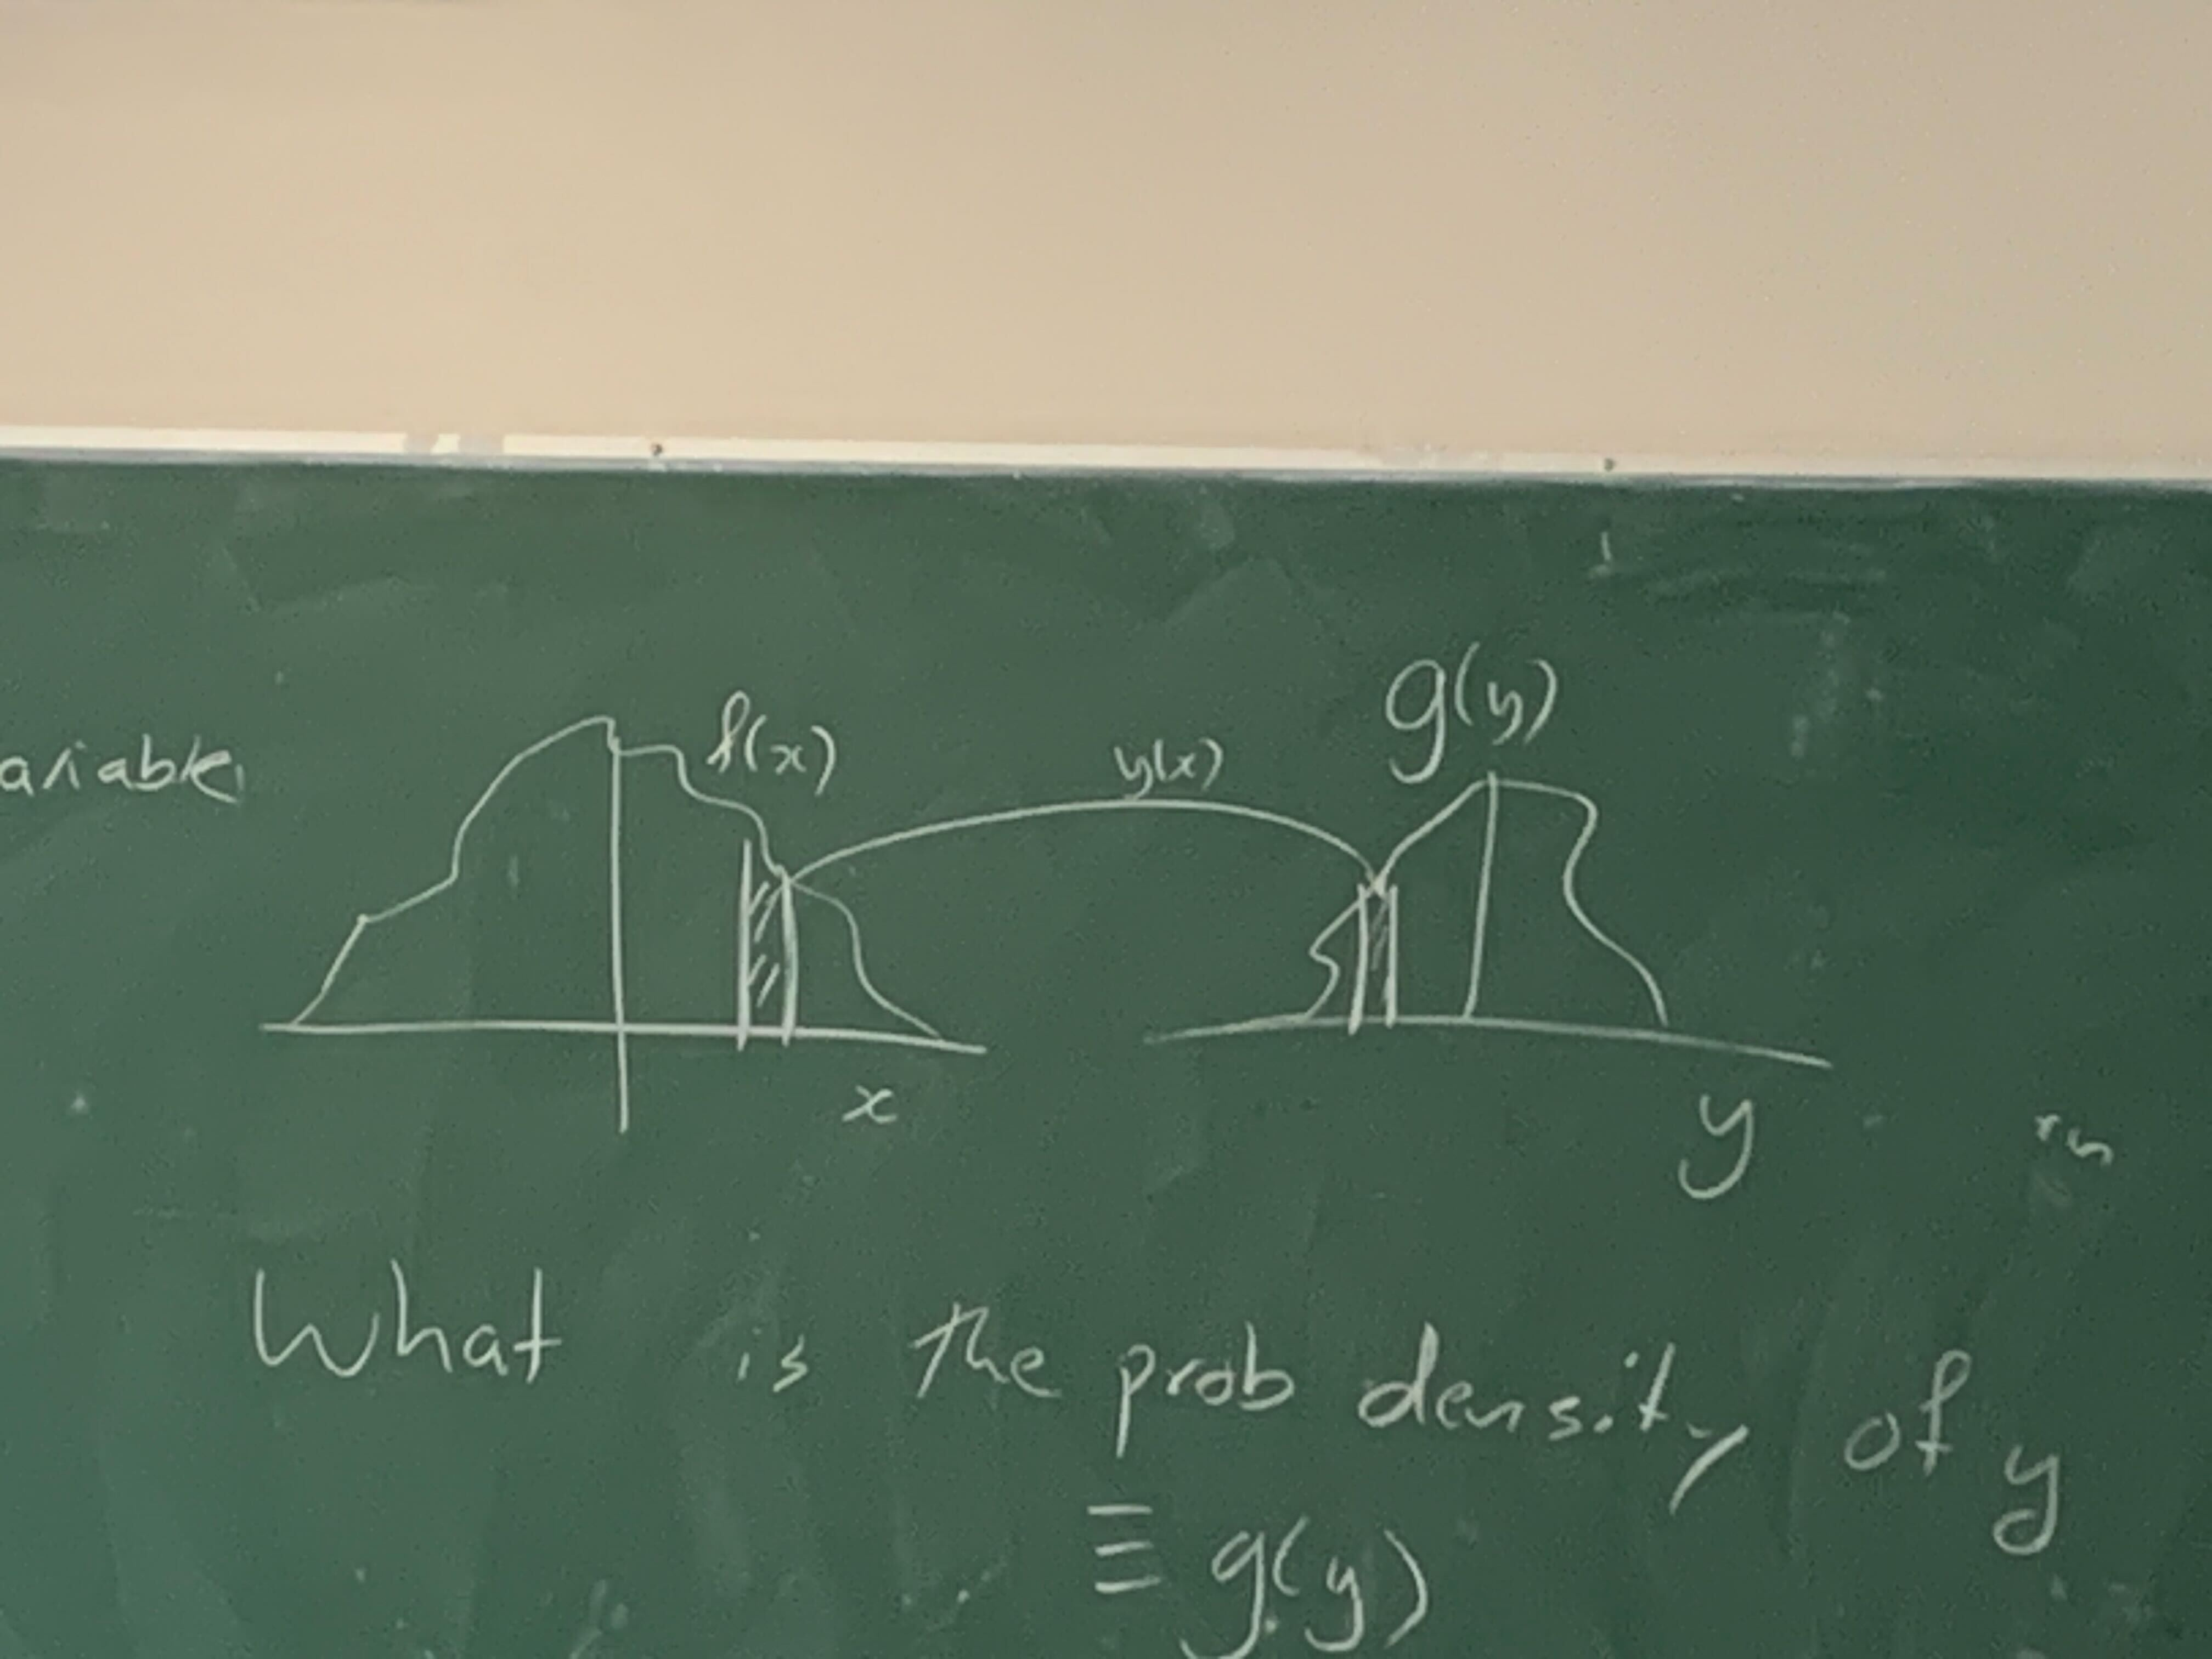
\includegraphics[width=0.4\textwidth]{Images/lec4-fig1.jpg}
              \caption{1-to-1 function}
              \label{fig:fig1}
          \end{figure}

    \item What is the probability density of $y$, denoted $g(y)$?
    \item Conservation of probability:
    \item $f(x) dx = g(y) dy$
    \item $g(y) = f(x) \left| \frac{dx}{dy} \right|$
          \[ \boxed{ f(x) \left| \frac{dx}{dy} \right| = g(y) } \]
\end{itemize}

\subsection{Change of Variables: Non One-to-One Case}
\begin{itemize}
    \item If $y$ is not one-to-one: sum over all segments that map to the same $y$.
    \item Example: $f(x)$ uniform on $[0,1]$, $f(x) = 1$
    \item Let $y(x) = \frac{-1}{\lambda} \ln(x)$
    \item $\frac{dy}{dx} = \frac{-1}{\lambda x}$
    \item $\frac{dx}{dy} = -\lambda x$
    \item $-\lambda x = \ln{x}$
    \item $e^{-\lambda y} = x$
    \item $\lambda > 0 \Rightarrow \frac{dx}{dy} = - \lambda x = -\lambda e^{-\lambda y}$
    \item $ g(y) = f(x) \left| \frac{dx}{dy} \right| = 1 \cdot \lambda e^{-\lambda y} = \lambda e^{-\lambda y}$
\end{itemize}

\subsection{Multivariate Transformations and the Jacobian}
\begin{itemize}
    \item If we have variables $\{x_i\}$ and transform to new variables $\{y_i\}$:
    \item Region $\mathbb{R}$ in $x$-space maps to region $\mathbb{R'}$ in $y$-space.
          \[ \int_{\mathbb{R}} f(\vec{x}) d\vec{x} = \int_{\mathbb{R'}} f(\vec{x}(\vec{y}))(\vec{y}) \left| \pdv{\vec{x}}{\vec{y}} \right| d\vec{y} \]
          \[ g(\vec{y}) = f(\vec{x}(\vec{y})) \left| J \right| \]
    \item Where $\left|\pdv{\vec{x}}{\vec{y}} \right|$ is the Jacobian determinant of the transformation.
    \item Jacobian matrix $J$:
          \[ J = \begin{bmatrix}
                  \pdv{x_1}{y_1} & \pdv{x_1}{y_2} & \ldots & \pdv{x_1}{y_n} \\
                  \pdv{x_2}{y_1} & \pdv{x_2}{y_2} & \ldots & \pdv{x_2}{y_n} \\
                  \vdots         & \vdots         & \ddots & \vdots         \\
                  \pdv{x_n}{y_1} & \pdv{x_n}{y_2} & \ldots & \pdv{x_n}{y_n}
              \end{bmatrix} \]
\end{itemize}

\subsection{Example: Cartesian to Polar Transformation}
\begin{itemize}
    \item Change to polar coordinates:
    \item $x = r \cos{\theta}$
    \item $y = r \sin{\theta}$
    \item $P'(r, \theta) = ? = p(x,y) \left| \pdv{(x,y)}{(r,\theta)} \right|$

    \item $ \pdv{x}{r} = \cos{\theta}$
    \item $ \pdv{y}{r} = \sin{\theta}$
    \item $ \pdv{x}{\theta} = -r \sin{\theta}$
    \item $ \pdv{y}{\theta} = r \cos{\theta}$

    \item $J = \begin{bmatrix}
                  \cos{\theta} & -r \sin{\theta} \\
                  \sin{\theta} & r \cos{\theta}
              \end{bmatrix}$

    \item $ J = r \cos^2{\theta} + r \sin^2{\theta} = r$
    \item $p'(r, \theta) = \frac{r}{\pi} dr d\theta$
\end{itemize}


\newpage
\section{Tuesday, September 20th 2025}

\subsection{Propagation of Errors for a Single Variable}

\begin{itemize}
      \item Given $f(x)$ pdf, $\mu \equiv E(x)$, $\sigma^2 \equiv V(x) = E(x^2) - \mu^2$
      \item Know $f(x) \rightarrow g(y)$, given $y(x)$.
      \item Taylor expand $y(x)$ about mean $\mu$:
            \[ y(x) = y(\mu) + y'(\mu) (x - \mu) + \frac{1}{2!} y''(\mu) (x - \mu)^2 + \ldots \]
            \[ E(y(x)) ? \equiv \mu_y \]
            \[ E(y(x)) = E(y(\mu)) + y'(\mu) E(x - \mu) + \frac{1}{2!} y''(\mu) E((x - \mu)^2) + \ldots \]
            \[ = y(\mu) + y'(\mu) \cdot 0 + \frac{1}{2!} y''(\mu) V(x)+ \ldots \]

      \item To the 1st order:
            \[ \mu_y = E(y(x)) = y(\mu) = y(E(x)) \]
\end{itemize}

\subsection{Variance Propagation for a Single Variable}

\begin{itemize}
      \item Variance of $y$:
            \begin{align}
                  V(y) & = E((y(x)-E(y(x)))^2)                                               \\
                       & = E((y(x) - \mu_y)^2)                                               \\
                       & = E((y'(\mu)(x-\mu) + \frac{1}{2!} y''(\mu)(x-\mu)^2 + \ldots)^2)   \\
                       & = E(y'(\mu)^2 (x-\mu)^2 + y'(\mu) y''(\mu)(x-\mu)^3 + O((x-\mu)^4)) \\
                       & = y'(\mu)^2 V(x) + \ldots
            \end{align}

      \item Some relations:
            \begin{align*}
                  E(x) & \equiv \mu_x                                 \\
                  V(x) & \equiv \sigma_x^2                            \\
                  y    & = y(x)                                       \\
                  E(y) & \equiv \mu_y = y(\mu_x)                      \\
                  V(y) & \equiv \sigma_y^2 = (y'(\mu_x))^2 \sigma_x^2
            \end{align*}

            \[ \sigma_y = |y'(\mu_x)| \sigma_x \]

      \item Example: $ y = \frac{1}{x}$, $\dv{y}{x} = -\frac{1}{x^2}$
            \[ \sigma^2_y = \frac{1}{\mu_x^4} \sigma_x^2 \]
\end{itemize}

\subsection{Propagation of Errors for Multiple Variables}

\begin{itemize}
      \item Let us suppose we have $n$ variables $\{ x_i \}$, with pdf $f(\vec{x})$.
      \item Let $y_j = 1, 2, \ldots, m$ be $m$ functions of $x_i$.
      \item $y_j = y_j(x_1, x_2, \ldots, x_n)$
      \item $V_{ij}(x)_{n \times n}(\vec{x}) = \text{covariance matrix of } \{x_i\}$
      \item $V_{ij}(\vec{x}) = E((x_i - \mu_i)(x_j - \mu_j))$
      \item Taylor expand each $y_j$: $\vec{\mu} = (\mu_1, \mu_2, \ldots, \mu_n)$
      \item $y_j(\vec{x}) = y_j(\vec{\mu}) + \sum_i \left. \pdv{y_j}{x_i} \right|_{\vec{\mu}} (x_i - \mu_i) + \frac{1}{2!} \sum_{i,k} \left. \pdv[2]{y_j}{x_i}{x_k} \right|_{\vec{\mu}} (x_i - \mu_i)(x_k - \mu_k) + \ldots$
      \item $E(y_j(\vec{x})) = E(y_{j}(\vec{\mu})) + \sum \pdv{y_j}{x_i} E(x_i - \mu_i) + \ldots = y_j(\vec{\mu})$
\end{itemize}

\subsection{Covariance Propagation for Functions of Multiple Variables}

\begin{itemize}
      \item Covariance between $y_k$ and $y_l$:
            \[ E((y_k - \mu_{y_k})(y_l - \mu_{y_l})) \]
            \[ = E((y_k-y_k(\mu))(y_l - y_l(\mu))) \]
            \[ = E\left( \sum_i \left. \pdv{y_k}{x_i}\right|_{\mu} (x_i - \mu_i) \sum_j \left. \pdv{y_l}{x_j}\right|_{\mu} (x_j - \mu_j) \right) \]
            \[ = \sum_{i,j} \left. \pdv{y_k}{x_i}\right|_{\mu}  \left. \pdv{y_l}{x_j} \right|_{\mu} E((x_i - \mu_i)(x_j - \mu_j)) \]

            \[ \boxed{ V_{kl}(\vec{y})_{m \times m} = \sum_{i,j} \left. \pdv{y_k}{x_i}\right|_{\vec{\mu}}  \left. \pdv{y_l}{x_j} \right|_{\vec{\mu}} V_{ij}(\vec{x})_{n \times n} }\]

      \item Example: $x, y$ random variables,
            \[ V(x,y) = \begin{bmatrix}
                        V_{xx} & V_{xy} \\[6pt]
                        V_{yx} & V_{yy}
                  \end{bmatrix} = \begin{bmatrix}
                        \sigma_x^2                  & \rho_{xy} \sigma_x \sigma_y \\[6pt]
                        \rho_{xy} \sigma_x \sigma_y & \sigma_y^2
                  \end{bmatrix} \]
      \item $z = x + y$
      \item $V(z) = \sigma_z^2 = \left(\pdv{z}{x} \right)^2 V_{xx} + 2  \pdv{z}{x} \pdv{z}{y} V_{xy} + \left(\pdv{z}{y} \right)^2 V_{yy}$
      \item $ = \sigma_x^2 + 2 \rho_{xy} \sigma_x \sigma_y + \sigma_y^2$
      \item If $x_i$ are uncorrelated,
            \[ V_{ij} = \sigma_{i,j} \sigma_{i}^2 = \begin{bmatrix}
                        \sigma_1^2 & 0          \\[6pt]
                        0          & \sigma_2^2
                  \end{bmatrix} \]
            \[ V_{kl}(\vec{y}) = \sum_i \left. \pdv{y_k}{x_i}\right|_{\mu}  \left. \pdv{y_l}{x_i} \right|_{\mu} V_{ii}(\vec{x}) \]
            \[ \text{variance } V_{kk} = \sum_i \left(\pdv{y_k}{x_i} \right)^2 \sigma_i^2 \]
\end{itemize}

\subsection{Examples of Error Propagation in Measurements}

\begin{itemize}
      \item Example: Measuring resistances. $x_i$ independent, $z = x + y$, $x=R_1$ resistor value, $y=R_2$ resistor value, $z=R_{\text{tot}}$ total resistance.
      \item $R_1 \pm \sigma_{R_1}$
      \item Convention is to use $\sqrt{V(R)}$ as uncertainty.
      \item For a good measuring device, $E(R) = R_{\text{true}}$ $\leftarrow$ unbiased.
      \item $V(R) = \text{small}$
      \item $R_1 \pm \sigma_{R_1}$, $R_2 \pm \sigma_{R_2}$, then $\sigma_{R_{\text{tot}}} = \sqrt{\sigma_{R_1}^2 + \sigma_{R_2}^2}$
      \item $R = R_{\text{tot}} = R_1 + R_2$
      \item $z = xy$, like $I, R$
      \item $\sigma_z^2 = \left(\pdv{z}{x} \right)^2 \sigma_x^2 + \left(\pdv{z}{y} \right)^2 \sigma_y^2 = y^2 \sigma_x^2 + x^2 \sigma_y^2$
            \[ \boxed{ \left(\frac{\sigma_z}{z} \right)^2 = \left(\frac{\sigma_x}{x} \right)^2 + \left(\frac{\sigma_y}{y} \right)^2 } \]
\end{itemize}

\subsection{Matrix Formulation of Linear Error Propagation}

\begin{itemize}
      \item Formula is exact if transformation of variables is linear.
      \item $\vec{y} = A \vec{x}$, $A$ is $m \times n$ matrix, $\vec{x}$ is $n \times 1$, $\vec{y}$ is $m \times 1$.
      \item $\pdv{y_k}{x_i} = \text{constant} \Rightarrow$ higher order terms in Taylor expansion are $0$
      \item $V_{kl}(\vec{y}) = \sum_{i,j} \pdv{y_k}{x_i} \pdv{y_l}{x_j} V_{ij}(\vec{x})$
      \item Matrix notation:
      \item $V_{kl}(\vec{y})  = \sum_{i,j} A_{ki} A_{lj} V_{ij}(\vec{x})$
      \item $ = \sum_{i,j} A_{ki} V_{ij}(\vec{x}) A_{lj}$
      \item $ = \sum_{i,j} A_{ki} V_{ij} (A^T)_{jl}$
      \item $ = (A V(\vec{x}) A^T)_{kl}$
            \[ \boxed{ V(\vec{y})_{m \times m} = A_{m \times n} V(\vec{x})_{n \times n} A^T_{n \times m} } \]
\end{itemize}

\subsection{Variance of the Arithmetic Mean}

\begin{itemize}
      \item Example: Arithmetic mean. Let $x_i = n$ identical independent variables with $V(x_i) = \sigma_x^2$
      \item Set $\bar{x} = \frac{1}{n} \sum_{i=1}^{n} x_i$
      \item Recall that $V(a x) = a^2 V(x)$
      \item $V(\bar{x}) = V\left(\frac{1}{n} \sum_{i=1}^{n} x_i\right) = \frac{1}{n^2} V\left(\sum_{i=1}^{n} x_i\right) = \frac{1}{n^2} \sum_{i=1}^{n} V(x_i) = \frac{1}{n^2} n \sigma_x^2 = \frac{\sigma_x^2}{n}$
      \item If variables are different $\sigma_i^2$: $n$ measurements
      \item $\bar{x} = \frac{1}{n} \sum_{i=1}^{n} x_i$
      \item $V(\bar{x}) = \frac{1}{n^2} \sum_{i=1}^{n} V(x_i) = \frac{1}{n^2} \sum_{i=1}^{n} \sigma_i^2$
      \item $\sigma_{\bar{x}} = \frac{1}{n} \sqrt{\sum_{i=1}^{n} \sigma_i^2}$
\end{itemize}

\subsection{Example: Measuring the Period of a Sine Wave}

\begin{itemize}
      \item Example: Measure period of sine wave on scope.
      \item $T = \Delta t = t_2 - t_1$
      \item $\sigma_T^2 = \left(\pdv{\Delta t}{t_1} \right)^2 \sigma_{t}^2 + \left(\pdv{\Delta t}{t_2} \right)^2 \sigma_{t}^2 = \sigma_t^2 + \sigma_t^2 = 2 \sigma_t^2$
      \item Measure $N$ cycles, $T = \frac{1}{N} \Delta t $
      \item $ \sigma_{T^2} = \frac{1}{N^2} \sigma_{\Delta t}^2 = \frac{2}{N^2} \sigma_t^2$
\end{itemize}


\newpage
\section{Tuesday, September 25th 2025}

\subsection{Covariance Transformation Under Linear Transformations}

\begin{itemize}
      \item Linear transformation:
            \[ \vec{y} = A\vec{x} \]
            \[ V_{kl}(\vec{y}) = \sum_{i,j} \pdv{y_k}{x_i} \pdv{y_l}{x_j} V_{ij}(\vec{x}) \]
      \item Linear $y_k = \sum A_{kj} x_j$
      \item then
            \[ V_{kl}(\vec{y}) = \sum_{i,j} A_{ki} A_{lj} V_{ij}(\vec{x}) \]
      \item or in matrix form
            \[ V(\vec{y}) = \left(A V(\vec{x}) A^T\right)_{kl} \]

            \subsubsection*{Diagonalization via Eigenvectors}

      \item If $\hat{e}_i$ are the eigenvectors of $V$, then
            \[ V (\vec{x})\hat{e}_i = \lambda_i \hat{e}_i \]
      \item Form:
            \[ A = \begin{pmatrix}
                        \hat{e}_1 \\
                        \ldots    \\
                        \hat{e}_n
                  \end{pmatrix}
                  = \begin{pmatrix}
                        \hat{e}_{11} & \hat{e}_{12} & \ldots & \hat{e}_{1n} \\
                        \ldots       & \ldots       & \ldots & \ldots       \\
                        \hat{e}_{n1} & \hat{e}_{n2} & \ldots & \hat{e}_{nn}
                  \end{pmatrix} \]
      \item then
            \[ A^T A = I \]
      \item then:
            \[ V A^T = V \begin{pmatrix}
                        \hat{e}_1 & \ldots \\
                        \ldots    & \ldots \\
                        \hat{e}_n & \ldots
                  \end{pmatrix} = \begin{pmatrix}
                        \lambda_1 \hat{e}_{11} & \ldots & \lambda_n \hat{e}_{n1} \\
                        \ldots                 & \ldots & \ldots                 \\
                        \lambda_1 \hat{e}_{1n} & \ldots & \lambda_n \hat{e}_{nn}
                  \end{pmatrix} \]

      \item Then:
            \[ A V A^T = \begin{pmatrix}
                        \hat{e}_{11} & \ldots & \hat{e}_{1n} \\
                        \ldots       & \ldots & \ldots
                  \end{pmatrix}
                  \begin{pmatrix}
                        \lambda_1 \hat{e}_{11} & \ldots          \\
                        \ldots                 & \ldots & \ldots \\
                        \lambda_1 \hat{e}_{1n} & \ldots
                  \end{pmatrix}
                  = \begin{pmatrix}
                        \lambda_1 & 0         & \ldots & 0         \\
                        0         & \lambda_2 & \ldots & 0         \\
                        \ldots    & \ldots    & \ldots & \ldots    \\
                        0         & 0         & \ldots & \lambda_n
                  \end{pmatrix} \]

      \item Then:
            \[ AVA^T = V(\vec{y}) = \begin{pmatrix}
                        \sigma_1^2 & 0          & \ldots & 0          \\
                        0          & \sigma_2^2 & \ldots & 0          \\
                        \ldots     & \ldots     & \ldots & \ldots     \\
                        0          & 0          & \ldots & \sigma_n^2
                  \end{pmatrix} \]
\end{itemize}

\subsection{The Binomial Distribution}

\begin{itemize}
      \item Consider an experiment with two outcomes.
      \item E.g. coin flips, selecting a ball with 2 possible colours, etc.
      \item One trial is called a Bernoulli trial.

            \subsubsection*{Bernoulli Trials and Sampling Methods}

      \item Example -- Method 1: You have an urn filled with $N$ balls. Some are red (R), some are blue (B).
      \item (0) What is your estimate of $n_R$, $n_B$, or $f = n_R/N$ or $p$ of drawing R?
      \item (1) You pick a ball: R. Q: estimate of $p = n_R/N$?
      \item (2) You pick another without replacing 1st ball: get R.
      \item (3) R
      \item (4) Get B
      \item This is a question about this ONE urn.

      \item Now Method 2: you draw red, and you PUT IT BACK. You repeat this several times.
      \item Now Method 3: We have an infinite source of balls with fraction $p$ red and $(1-p)$ blue.
            \begin{align*}
                  P(R) & = p   \\
                  P(B) & = 1-p
            \end{align*}

            \subsubsection*{Derivation of the Binomial Probability}

      \item Make infinite number of urns all with $N$ balls, with fraction $p$ red and $(1-p)$ blue.
      \item Open all, count $n_R$ red balls, $n_B$ blue balls.
      \item In our case we have $N$ balls, prob $p=R$ and $1-p=q=B$.
      \item Prob of getting sequence RRB is:
            \[ P(RRB) = p \cdot p \cdot (1-p) = p^2 (1-p) \]
      \item If we don't care about order, then:
            \[ P(RRB) = P(RBR) = P(BRR) = p^2 (1-p) \]
      \item There are 3 ways of ordering RRB, so total probability is:
            \[ P(2R,1B) = 3 p^2 (1-p) = 3 p^2 q \]
      \item Number of ways to choose $r$ items from $N$ is:
            \[ \binom{N}{r} = \frac{N!}{r!(N-r)!} \]
      \item Probability of getting exactly $r$ R out of $N$:
            \[ P_r = \binom{N}{r} p^r (1-p)^{N-r} = B(r;N,p) \]
      \item This is called the Binomial distribution and applies to anything where there are 2 outcomes ($A, \bar{A}$).

            \subsubsection*{Mean and Variance of the Binomial Distribution}

      \item Want mean, $\sigma$
            \begin{align*}
                  E(r) & = \sum_{r=0}^n r P_r = \sum_{r=0}^n r \binom{n}{r} p^r (1-p)^{n-r} \\
                       & = \sum_{r=0}^n r \frac{n!}{r!(n-r)!} p^r (1-p)^{n-r}               \\
                       & = \sum_{r=1}^n \frac{n!}{(r-1)!(n-r)!} p^r (1-p)^{n-r}             \\
                       & = np \sum_{r=1}^n \frac{(n-1)!}{(r-1)!(n-r)!} p^{r-1} (1-p)^{n-r}
            \end{align*}
      \item Change sum $r' = r-1$ $\rightarrow n' = n-1$
            \begin{align*}
                  E(r) & = np \sum_{r'=0}^{n-1} \frac{(n-1)!}{r'!(n-1-r')!} p^{r'} (1-p)^{(n-1)-r'} \\
                       & = np \sum_{r'=0}^{n-1} \binom{n-1}{r'} p^{r'} (1-p)^{n'-r'}                \\
                       & = np \cdot 1 = np
            \end{align*}

      \item from:
            \[ (p+q)^n = \sum_{r=0}^n \binom{n}{r} p^r q^{n-r} \]
            \[ (p+1-q)^n = 1^n = 1 \]
            \[ E(r) = np \]
      \item This is what we want!
      \item Now:
            \[ V(r) = \sum r^2 p_r - E(r)^2 = \sum r^2 p_r - n^2 p^2 \]
      \item Slightly easier to calculate:
            \[ \sum r(r-1) p_r = \sum_{r=0}^n r(r-1) \frac{n!}{r!(n-r)!} p^r (1-p)^{n-r} = \sum_{r=2}^n \frac{n!}{(r-2)!(n-r)!} p^r q^{n-r} \]
            \[ = n(n-1) p^2 \sum_{r=2}^n \frac{(n-2)!}{(r-2)!(n-r)!} p^{r-2} q^{n-r} \]
      \item Sub $r' = r-2$
            \[ = n(n-1) p^2 \sum_{r'=0}^{n-2} \binom{n-2}{r'} p^{r'} q^{(n-2)-r'} \]
            \[ = n(n-1)p^2 \cdot 1 = n(n-1)p^2 \]
            \[ = n^2 p^2 - np^2 \]
      \item Such that:
            \[ \boxed{V(r) = \sum r^2 p_r - n^2 p^2 } = np (1 - p) = npq \]

            \subsubsection*{Applications to Histograms and Counting Statistics}

      \item Why is this important? Histograms are often Binomially distributed.
      \item Data either falls $A$: falls in bin, or $\bar{A}$: does not fall in bin.
      \item $p =$ probability of falling in $i$th bin.
      \item $+n$ entries, e.g. students in class, histogram = grades.
      \item Expected number of entries is $np$.
      \item Plot of taking distribution several times and checking how many fall in bin $i$ and then plotting that distribution is Binomial.
      \item Usually you have 1 histogram.
      \item Look at entries in bin $i$ -- $n_i/n$ = fraction of entries in bin $i$.
      \item Estimator $p = n_i/n$.
      \item Expect if you repeated $\Rightarrow$ $n_i$ would follow Binomial distribution with mean $\sigma_i = \sqrt{n p q}$ and $V_i = \sigma_i^2 = np (1 - p)$.
      \item \[ p = \frac{n_i}{n} \]
      \item \[ \boxed{\sigma_i = \sqrt{n_i \left(1 - \frac{n_i}{n}\right)}} \approx \sqrt{n_i} \text{ if } n \gg n_i \]

      \item Notes: we do know the total number $n$, how often is it in bin $i$.
      \item HW: given the distribution, how many times $n$ do I need to do it to get that.
      \item $r$ fixed $n$, vs. $n$ fixed $r$.
\end{itemize}


\newpage
\section{Lecture 7}

Thursday, October 2nd 2025

\subsection{Review of the Binomial Distribution and Its Properties}

\begin{itemize}
      \item Recall last time:
            \[ B(r, n, p) = \binom{n}{r} p^r (1-p)^{n-r} \]
            \[ E(r) = np = \mu \]
            \[ V(r) = np(1-p) = \sigma^2 \]
            \[ r = \sqrt{np(1-p)} \]
            \[ p = \frac{\mu}{n} \]

      \item $\epsilon = \frac{r}{n}$
      \item Number of detections (people often forget the $(1-p)$ term):
            \[ n \epsilon \pm \sqrt{n \epsilon (1-\epsilon)} \]

      \item $\sigma_{\epsilon} = \frac{1}{n} \sigma_r = \frac{1}{n} \sqrt{r \left(1-\frac{r}{n}\right)} = \frac{1}{\sqrt{n}} \sqrt{\epsilon (1-\epsilon)}$

      \item Standardized skewness:
            \[ E \left[ \left( \frac{x-\mu}{\sigma} \right)^3 \right] = \frac{1-2p}{\sqrt{np(1-p)}} \]

      \item Excess kurtosis:
            \[ \frac{1-6p(1-p)}{np(1-p)} \]
\end{itemize}

\subsection{Bernoulli Distribution as a Special Case of the Binomial}

\begin{itemize}
      \item Bernoulli Distribution: Binomial with $n=1$.
            \[ B(r, n=1, p) = P_r = \binom{1}{r} p^r (1-p)^{1-r} = p^r (1-p)^{1-r} \]
            \[ P_0 = 1 - p \]
            \[ P_1 = p \]
            \[ \mu  = E(r) = np = p \]
            \[ V = \sigma^2 = np(1-p) = p(1-p) \]
            \[ E(r^k) = \sum_{r=0}^{1} r^k P_r = 0^k (1-p) + 1^k p = p \]
      \item Central moments: $E[(r-p)^k]$
\end{itemize}

\subsection{Negative Binomial and Geometric Distributions}

\begin{itemize}
      \item Negative Binomial: How many $n$ to get $r$ successes.
      \item Geometric distribution: negative binomial with $r=1$ (number of trials to get first success).
            \[ G(n,p) = p (1-p)^{n-1} \]
      \item Example: Roll a die with $p(i) = 1/6$ (success = get 4)
            \[ E(n) = \frac{1}{p} = 6 \]
      \item $P(n \le 5) = 0.598$
      \item $P(n \ge 7) = 0.335$
\end{itemize}

\subsection{Samples and the Concept of an Ensemble}

\begin{itemize}
      \item Samples: A set of $N$ draws/trials from a pdf $p(x)$, $\{ P_r \}$, is called a \textbf{sample} of size $N$: $\{x_i \}_{i=1}^N$.
      \item Orthodox statistics: your sample is one of many possible, and we can answer questions about the \textbf{ensemble} of samples.
      \item Samples:
            \begin{itemize}
                  \item 1: $\{ x_{1i} \}_{i=1}^N$ from pdf $p(x)$
                  \item 2: $\{ x_{2i} \}_{i=1}^N$ from pdf $p(x)$
                  \item ...
                  \item M
            \end{itemize}
      \item $p(x|\mu, \sigma)$
      \item $p$ = probability of $H$ (heads), $q = 1 - p$ = probability of $T$ (tails)
      \item These are limits: $p = \lim_{n\rightarrow \infty} \frac{n_H}{n}$
      \item Flip 10 times: exactly $2^{10} = 1024$ possible outcomes
            \[ S_1 = \{ HHHHHHHHHH \} \]
            \[ S_2 = \{ HTHHHHHHHH \} \]
            \[ \ldots \]
      \item Given true $p$, calculate probability of any $S_i$:
            \[ P_i = \lim_{N\rightarrow \infty} \frac{n_i}{N} \]
      \item From the pdf probability, select $k$ samples from a sample space of size $F$.
      \item Science/statistics infers from sample space $\mathcal{R}$ to get $p(x)$.
      \item Not purely deductive: $\infty$ number of pdfs map to one sample.
      \item Inductive: If sample pdf is more likely.
      \item Sample HHTHT ... known, from it we try to infer $p = p_H$.
\end{itemize}

\subsection{Poisson Distribution as a Limit of the Binomial}

\begin{itemize}
      \item Poisson Distribution: limit of binomial for large $n$, small $p$.
      \item
            \[ B(r,n,p) = \binom{n}{r} p^r (1-p)^{n-r} \]
      \item Let $n \rightarrow \infty$, $p \rightarrow 0$ such that $np = \mu$ is constant.
      \item Stirling approximation:
            \[ n! \approx \sqrt{2 \pi n}  n^n e^{-n} \]
      \item Then:
            \[ B(r,n,p) = \frac{n!}{r!(n-r)!} p^r (1-p)^{n-r} \]
      \item $r$ is finite, $n \rightarrow \infty$, $n-r \rightarrow \infty$

            \begin{align*}
                  B(r,n,p) & = \frac{1}{r!} \frac{\sqrt{2 \pi n}}{\sqrt{2 \pi (n-r)}} \frac{n^n e^{-n}}{(n-r)^{n-r} e^{-(n-r)}} \left(\frac{\mu}{n}\right)^r \left(1-\frac{\mu}{n}\right)^{n-r}          \\
                           & = \frac{1}{r!} \sqrt{\frac{n}{n-r}} \left( \frac{n}{n-r} \right)^{n-r} \frac{\mu^r}{e^r} \frac{\left(1-\frac{\mu}{n}\right)^{n}}{\left(1-\frac{\mu}{n}\right)^r}            \\
                           & = \frac{1}{r!} \sqrt{\frac{n}{n-r}} \frac{(1-\frac{r}{n})^r}{(1-\frac{r}{n})^{n}} \frac{\mu^r}{e^r} \frac{\left(1-\frac{\mu}{n}\right)^{n}}{\left(1-\frac{\mu}{n}\right)^r} \\
            \end{align*}

      \item $n\rightarrow \infty$, $\sqrt{\frac{n}{n-r}} \rightarrow 1$
      \item $\left(1-\frac{\mu}{n}\right)^n \rightarrow e^{-\mu}$
      \item $\left(1-\frac{\mu}{n}\right)^r \rightarrow 1$
      \item Then:
            \[ \lim_{n\rightarrow \infty,\, np = \mu} B(r,n,p) = \frac{1}{r!} \mu^r e^{-\mu} = P(r|\mu) = \text{Poisson} \]
\end{itemize}

\subsection{Poisson Process and Radioactive Decay}

\begin{itemize}
      \item Consider radioactive decay of some atoms:
            \begin{enumerate}
                  \item Any time interval $[t, t+dt]$ contains at most one decay.
                  \item Probability of a decay occurring in this interval is proportional to $dt$.
                  \item Whether or not an atom decays in the interval is independent of any other non-overlapping interval.
            \end{enumerate}

      \item From (1) and (2):
            \[ P_d(dt) = \lambda dt \]
      \item Probability of no decay in interval:
            \[ P_0(dt) = 1 - \lambda dt \]
      \item Probability of no decay by time $t + dt$:
            \begin{align*}
                  P_0(t+dt)          & = P_0(t) P_0(dt)                         \\
                                     & = P_0(t) (1 - \lambda dt)                \\
                  P_0(t+dt) - P_0(t) & = -\lambda P_0(t) dt                     \\
                  \frac{dP_0(t)}{dt} & = -\lambda P_0(t)                        \\
                  P_0(t)             & = P_0(0) e^{-\lambda t} = e^{-\lambda t}
            \end{align*}

      \item Probability of getting $r$ decays in time $t + dt$:
            \begin{align*}
                  P_r(t+dt)          & = P_r(t) P_0(dt) + P_{r-1}(t) P_d(dt)             \\
                                     & = P_r(t) (1 - \lambda dt) + P_{r-1}(t) \lambda dt \\
                  \frac{dP_r(t)}{dt} & = -\lambda P_r(t) + \lambda P_{r-1}(t)
            \end{align*}

      \item Solution to PDE:
            \[ P_r(t) = \frac{1}{r!} (\lambda t)^r e^{-\lambda t} \]
      \item Poisson distribution with $\mu = \lambda t$
\end{itemize}

\subsection{Moments and Variance of the Poisson Distribution}

\begin{itemize}
      \item Properties:
            \begin{align*}
                  E(r) & = \sum_{r=0}^{\infty} r P(r,\mu)                            \\
                       & = \sum_{r=0}^{\infty} r \frac{\mu^r}{r!} e^{-\mu}           \\
                       & = \mu e^{-\mu} \sum_{r=1}^{\infty} \frac{\mu^{r-1}}{(r-1)!} \\
                       & = \mu e^{-\mu} e^{\mu}                                      \\
                       & = \mu
            \end{align*}

      \item $V(r) = E(r^2) - \mu^2$
            \begin{align*}
                  E[r(r-1)] & = E(r^2) - \mu                                                \\
                            & = \sum_{r=2}^{\infty} r(r-1) \frac{\mu^r}{r!} e^{-\mu}        \\
                            & = \mu^2 e^{-\mu} \sum_{r=2}^{\infty} \frac{\mu^{r-2}}{(r-2)!} \\
                            & = \mu^2 e^{-\mu} e^{\mu} = \mu^2
            \end{align*}

      \item $E(r^2) - \mu = \mu^2$
      \item $V(r) = E(r^2) - \mu^2 = \mu$
      \item Binomial: $\mu = np$, $V(r) = np(1-p) = \mu$ for $p \rightarrow 0$ and $n \rightarrow \infty$.
\end{itemize}


\newpage
\section{Tuesday, October 7th, 2025}

\subsection{The Gaussian (Normal) Distribution}
\[
      G(x|\mu, \sigma) = \frac{1}{\sqrt{2 \pi} \sigma}
      e^{-\frac{(x - \mu)^2}{2 \sigma^2}}
\]

\subsection{The Standard Normal Distribution}
\[
      N(0,1) = \frac{1}{\sqrt{2 \pi}} e^{-\frac{x^2}{2}}
\]

\subsection{Example: Circular Symmetry (Darts on a Board)}
Distribution of darts:
\[
      f(x,y) = h(x) k(y)
\]
Transform to polar coordinates:
\[
      g(r,\theta) \approx f(x,y) = h(x)k(y), \qquad g(r,\theta) = g(r)
\]
\[
      \pdv{g}{\theta} = 0
      = \pdv{f}{x}\pdv{x}{\theta} + \pdv{f}{y}\pdv{y}{\theta}
\]
Coordinates:
\[
      x = r \cos\theta, \qquad y = r \sin\theta
\]
\[
      \pdv{x}{\theta} = -r \sin\theta = -y, \qquad
      \pdv{y}{\theta} = r \cos\theta = x
\]
Condition:
\[
      0 = h'(x) k(y)(-y) + h(x) k'(y) x
\]
\[
      \frac{h'(x)}{x h(x)} = \frac{k'(y)}{y k(y)} = a \quad (\text{constant})
\]
Solutions:
\[
      h(x) = c e^{a x^2}, \qquad k(y) = d e^{a y^2}
\]
\[
      f(x,y) = A e^{a(x^2+y^2)} = A e^{a r^2} \approx A e^{-r^2}
\]

\subsection{Expectation Value of a Gaussian}
\[
      E(x) = \mu = \frac{1}{\sqrt{2 \pi}\sigma}
      \int_{-\infty}^{\infty} x e^{-\frac{(x - \mu)^2}{2\sigma^2}} dx = \mu
\]

Useful identity:
\[
      \int_{-\infty}^{\infty} e^{-a x^2} dx = \sqrt{\frac{\pi}{a}}
\]

\subsection{Moments of the Gaussian}
The $n$th central moment:
\[
      \frac{1}{\sqrt{2 \pi}\sigma} \int_{-\infty}^{\infty} (x-\mu)^n
      e^{-\frac{(x-\mu)^2}{2\sigma^2}} dx
\]

- All odd moments vanish (symmetry about $\mu$).

Define
\[
      I_0(a) = \int_{-\infty}^{\infty} e^{-a y^2} dy = \sqrt{\frac{\pi}{a}}
\]

Differentiation rule:
\[
      \dv[^n]{I_0(a)}{a} = (-1)^n \frac{(2n)!}{n!} \frac{I_0(a)}{(2a)^n}
\]

\subsection{Variance of the Gaussian}
Let $y = x-\mu$. Then
\[
      V(y) = V(x) = \frac{1}{\sqrt{2 \pi}\sigma}
      \int_{-\infty}^{\infty} y^2 e^{-\frac{y^2}{2\sigma^2}} dy
\]
\[
      = -\dv{I_0(a)}{a}\Bigg|_{a=\frac{1}{2\sigma^2}} = \sigma^2
\]

\subsection{Kurtosis of the Gaussian}
Fourth central moment:
\[
      \int y^4 e^{-a y^2} dy = \frac{d^2 I_0(a)}{d a^2}\frac{1}{4 a^2}
\]
Evaluates to:
\[
      E\!\left[\left(\frac{x-\mu}{\sigma}\right)^4\right] = 3
\]
Thus the Gaussian kurtosis = 3.
- Excess kurtosis = 0.
- Distributions with $>3$ have “fat tails.”

\subsection{Poisson Distribution and Gaussian Limit}
\[
      P(r|\lambda) = \frac{1}{r!} \lambda^r e^{-\lambda}
\]
For large $r$, Stirling approximation:
\[
      r! \approx \sqrt{2 \pi r} \left(\frac{r}{e}\right)^r
\]
\[
      \log P(r|\lambda) = -\log(r!) + r\log\lambda - \lambda
\]

Expanding around $r \approx \lambda$ leads to Gaussian limit with variance $\lambda$:
\[
      P(r|\lambda) \approx
      \frac{1}{\sqrt{2 \pi \lambda}} e^{-\frac{(r-\lambda)^2}{2\lambda}}
\]

\subsection{Central Limit Theorem (CLT)}
Let $x_1,\dots,x_n$ be independent random variables with
mean $\mu$, variance $\sigma^2$. Define sample mean
\[
      \bar{x} = \frac{1}{n} \sum_{i=1}^n x_i
\]
Then as $n \to \infty$:
\[
      \bar{x} \sim \mathcal{N}\!\left(\mu,\; \frac{\sigma^2}{n}\right)
\]

\subsection{Cumulative Distribution Function of a Gaussian}
\[
      F(x) = \int_{-\infty}^x G(y|\mu,\sigma) dy
\]

Define error function:
\[
      \text{erf}(t) = \frac{2}{\sqrt{\pi}} \int_0^t e^{-y^2} dy,
      \qquad
      \text{erfc}(t) = 1 - \text{erf}(t) = \frac{2}{\sqrt{\pi}} \int_t^\infty e^{-y^2} dy
\]

\subsection{Gaussian Confidence Intervals}
\begin{itemize}
      \item $1\sigma$: $68.27\%$
      \item $2\sigma$: $95.45\%$
      \item $3\sigma$: $99.73\%$
      \item $5\sigma$: $99.99994\%$
\end{itemize}

\subsection{Estimators}
Given a sample of size $n$, an \emph{estimator} is any function designed to estimate a property of the true pdf from which the samples were drawn.


\newpage
\section{Thursday, October 9th 2025}

\subsection{Properties of Estimators}
\begin{itemize}
      \item Consistent: $\lim_{n \rightarrow \infty} \hat{a} = a$
      \item Unbiased: $\mathbb{E}[\hat{a(x)}] = a$
      \item Efficient: smallest variance of all unbiased estimators
\end{itemize}

\subsection{Example: Measurements and Models}
\begin{itemize}
      \item Let $x_1, x_2, \ldots, x_n$ be $n$ measurement points.
      \item Example applications: number of elements in a histogram bin, position of hits in a detector.
      \item $y_i$ are the measured values at each $x_i$, with variances $V(y_i) = \sigma_i^2$.
      \item Suppose we suspect a model for the histogram shape (e.g.\ linear background $+$ Gaussian signal):
            \[
                  \text{Number of entries} = m x_i + b + A e^{-\frac{(x_i - \mu)^2}{2\sigma^2}}
            \]
      \item More generally, assume a function $f(x, \vec{\theta})$ with parameters $\vec{\theta}$.
\end{itemize}

\subsection{Least Squares Estimation}
\begin{itemize}
      \item The best estimate for $\vec{\theta}$ is the value that minimizes the chi-squared:
            \[
                  \chi^2 = \sum_{i=1}^{n} \frac{(y_i - f(x_i, \vec{\theta}))^2}{\sigma_i^2}.
            \]
      \item Condition for minimization:
            \[
                  \pdv{\chi^2}{\theta_j} = 0.
            \]
      \item Equivalent system of equations:
            \[
                  \sum_{i=1}^{n} \frac{(y_i - f(x_i, \vec{\theta}))}{\sigma_i^2}
                  \pdv{f(x_i, \vec{\theta})}{\theta_j} = 0.
            \]
\end{itemize}

\subsection{Straight Line Fit}
\begin{itemize}
      \item For $f(x_i, \vec{\theta}) = m x_i + b$, with $\vec{\theta} = (m, b)$:
            \[
                  \chi^2 = \sum_{i=1}^{n} \frac{(y_i - (m x_i + b))^2}{\sigma_i^2}.
            \]
      \item Normal equations from minimization:
            \[
                  \pdv{\chi^2}{m} = -2 \sum_{i=1}^{n} \frac{(y_i - (m x_i + b))}{\sigma_i^2} x_i = 0,
            \]
            \[
                  \pdv{\chi^2}{b} = -2 \sum_{i=1}^{n} \frac{(y_i - (m x_i + b))}{\sigma_i^2} = 0.
            \]
      \item Two equations, two unknowns. Can be written in matrix form:
            \[
                  \begin{bmatrix}
                        S_{xx} & S_x \\
                        S_x    & S_1
                  \end{bmatrix}
                  \begin{bmatrix}
                        m \\
                        b
                  \end{bmatrix}
                  =
                  \begin{bmatrix}
                        S_{xy} \\
                        S_y
                  \end{bmatrix},
            \]
            where
            \[
                  S_{xx} = \sum_i \frac{x_i^2}{\sigma_i^2}, \quad
                  S_x = \sum_i \frac{x_i}{\sigma_i^2}, \quad
                  S_1 = \sum_i \frac{1}{\sigma_i^2},
            \]
            \[
                  S_{xy} = \sum_i \frac{x_i y_i}{\sigma_i^2}, \quad
                  S_y = \sum_i \frac{y_i}{\sigma_i^2}.
            \]
\end{itemize}

\subsection{Generalized Least Squares with Covariance Matrix}
\begin{itemize}
      \item In general, for non-diagonal covariance matrix $V$ of $y_i$:
            \[
                  \chi^2 = \sum_{i=1}^{n} \sum_{j=1}^{n}
                  (y_i - f(x_i, \vec{\theta})) \, E_{ij} \, (y_j - f(x_j, \vec{\theta})),
            \]
            where $E = V^{-1}$ is the inverse covariance matrix.
      \item Linear case: if $f(x_i, \vec{\theta})$ is linear in $\theta$:
            \[
                  \vec{f} = A \vec{\theta}.
            \]
      \item Then
            \[
                  \chi^2 = (\vec{y} - A \vec{\theta})^T V^{-1} (\vec{y} - A \vec{\theta}).
            \]
      \item Minimization gives:
            \[
                  (A^T V^{-1} A) \vec{\theta} = A^T V^{-1} \vec{y},
            \]
            \[
                  \Rightarrow \vec{\theta} = (A^T V^{-1} A)^{-1} A^T V^{-1} \vec{y}.
            \]
\end{itemize}

\subsection{Covariance of the Estimated Parameters}
\begin{itemize}
      \item Propagation of covariance:
            \[
                  V(\vec{y}) = B V(\vec{x}) B^T.
            \]
      \item For parameter estimates:
            \[
                  V(\vec{\theta}) = (A^T V^{-1} A)^{-1}.
            \]
\end{itemize}

\subsection{Goodness of Fit}
\begin{itemize}
      \item The chi-squared statistic
            \[
                  \chi^2 = \sum_{i=1}^{n} \frac{(y_i - f(x_i, \vec{\theta}))^2}{\sigma_i^2}
            \]
            is distributed as $\chi^2$ with $n$ degrees of freedom if the $y_i$ are Gaussian.
      \item If the model is good, $\chi^2/\text{dof} \sim 1$; if the model is bad, $\chi^2/\text{dof} \gg 1$.
\end{itemize}



\newpage

\section{Lecture 10}

Tuesday, October 14th 2025

In this lecture, I start to not take all notes, instead I write down only the key points.

\subsection{Chi-Squared for Uncorrelated and Correlated Measurements}

\begin{itemize}
    \item Recall difference in chi-squared formula for uncorrelated and correlated measurements.
    \item Uncorrelated:
          \[
              \chi^2 = \sum_{i=1}^{n} \frac{(y_i - \mu_i)^2}{\sigma_i^2}
          \]
    \item Correlated (general case):
          \[
              \chi^2 = \sum_{i, j}^{n} (y_i - \mu_i) V^{-1}_{ij} (y_j - \mu_j)
          \]
          where $V^{-1}$ is the inverse of the covariance matrix $V$.
\end{itemize}

\subsection{Covariance Matrix and Linear Transformations}

\begin{itemize}
    \item The covariance matrix is defined as
          \[
              V_{ij} = \mathrm{Cov}(y_i, y_j) = \langle (y_i - \mu_i)(y_j - \mu_j) \rangle .
          \]
    \item Suppose we apply a linear transformation $B$ to $\vec{y}$, where $B$ is an $n \times n$ matrix of eigenvectors that diagonalizes $V$.
    \item Define transformed variables:
          \[
              \vec{z} = B \vec{y}, \quad V_z = B V B^T, \quad \mu_z = B \mu_y .
          \]
    \item Then:
          \[
              \boxed{\chi^2(z) = \left( \vec{z} - \vec{\mu_z} \right)^T V_z^{-1} \left( \vec{z} - \vec{\mu_z} \right)}
          \]
\end{itemize}

\subsection{Modeling Data with Parameters}

\begin{itemize}
    \item Suppose we have a model
          \[
              y_i = f(x_i, \vec{\theta}),
          \]
          where $x_i$ are independent variables and $\vec{\theta}$ are model parameters.
    \item Example: $y_i = m x_i + b$, with $\sigma_i \neq \sigma_j$ (heteroscedastic errors).
    \item We want to find the best estimate of $\vec{\theta}$.
\end{itemize}

\subsection{Least Squares Estimation}

\begin{itemize}
    \item Define:
          \[
              \chi^2(\vec{\theta}) = \sum_{i=1}^{n} \frac{(y_i - f(x_i, \vec{\theta}))^2}{\sigma_i^2} .
          \]
    \item The best estimators for $\mu_i$ are $f(x_i|\vec{\theta})$ and
          \[
              \chi^2(\hat{\theta}) = \chi^2_{\text{min}} = \sum_i \left( \frac{y_i - f(x_i|\hat{\theta})}{\sigma_i} \right)^2 .
          \]
    \item Principle of least squares:
          \[
              \hat{\theta} = \text{arg min } \chi^2(\vec{\theta})
          \]
          i.e. the value of $\vec{\theta}$ that minimizes $\chi^2(\vec{\theta})$.
    \item Solution satisfies:
          \[
              \pdv{\chi^2}{\theta_j} = 0 .
          \]
\end{itemize}

\subsection{Distribution of Parameter Estimates}

\begin{itemize}
    \item Note: $\hat{\theta}$ is itself a random variable, with its own probability distribution.
    \item A different sample $\{x_i, y_i\}$ will lead to a different $\hat{\theta}$.
\end{itemize}

\subsection{Quadratic Expansion of chi-squared and Error Estimates}

\begin{itemize}
    \item For polynomial (linear in parameters) fits:
          \[
              f(x_i|\vec{\theta}) = (A \vec{\theta})_i .
          \]
    \item Then:
          \[
              \chi^2 = (\vec{y} - A \vec{\theta})^T V^{-1} (\vec{y} - A \vec{\theta})
          \]
          \[
              \chi^2 = (y_i - A_{im} \theta_m) V_{ij}^{-1} (y_j - A_{jn} \theta_n) .
          \]
    \item First derivative:
          \[
              \pdv{\chi^2}{\theta_k} = -2 (y_i - A_{im} \theta_m) V_{ij}^{-1} A_{jk} .
          \]
    \item Second derivative:
          \[
              \pdv{\chi^2}{\theta_k}{\theta_l} = 2 A_{il} V_{ij}^{-1} A_{jk} = 2 (A^T V^{-1} A)_{kl} .
          \]
\end{itemize}

\subsection{Covariance of Parameter Estimates}

\begin{itemize}
    \item For linear fits:
          \[
              V(\hat{\theta}) = (A^T V^{-1} A)^{-1} .
          \]
    \item For non-linear fits:
          \[
              V^{-1}(\hat{\theta}) = \frac{1}{2} \pdv[2]{\chi^2}{\theta_j}{\theta_k} \Big|_{\theta = \hat{\theta}} .
          \]
\end{itemize}


\newpage

\section{Thursday, October 16th 2025}

I was gone this day, so I copied notes from J. Liang.

\subsection{Chi-Squared Minimization and Degrees of Freedom}

\begin{itemize}
      \item Degrees of Freedom (dof):
            \[
                  \chi^2(\theta) = (y - A \vec{\theta})^T V^{-1} (y - A \vec{\theta})
            \]
      \item At $\hat{\theta}$, $\chi^2$ is minimized:
            \[
                  \pdv{\chi^2}{\theta}\bigg|_{\theta = \hat{\theta}} = 0 =
                  F(\vec{y} | \vec{\theta}, \vec{x}) =
                  \begin{matrix}
                        F(\vec{y} | \theta_1, \vec{x}) \\
                        F(\vec{y} | \theta_2, \vec{x}) \\
                        \vdots                         \\
                        F(\vec{y} | \theta_k, \vec{x})
                  \end{matrix}
            \]
      \item i.e. for a linear fit $\vec{y} = A \vec{\theta}$ with $k$ equations:
            \[
                  \hat{\theta} = (A^T V^{-1} A)^{-1} (A^T V^{-1}) \vec{y}
            \]
      \item Think about it like this: If I know $n-k$ of the $y_i$'s, the remaining $k$ $y_i$'s are fixed. Their relations might be complex but they are fixed since we have $k$ equations.

            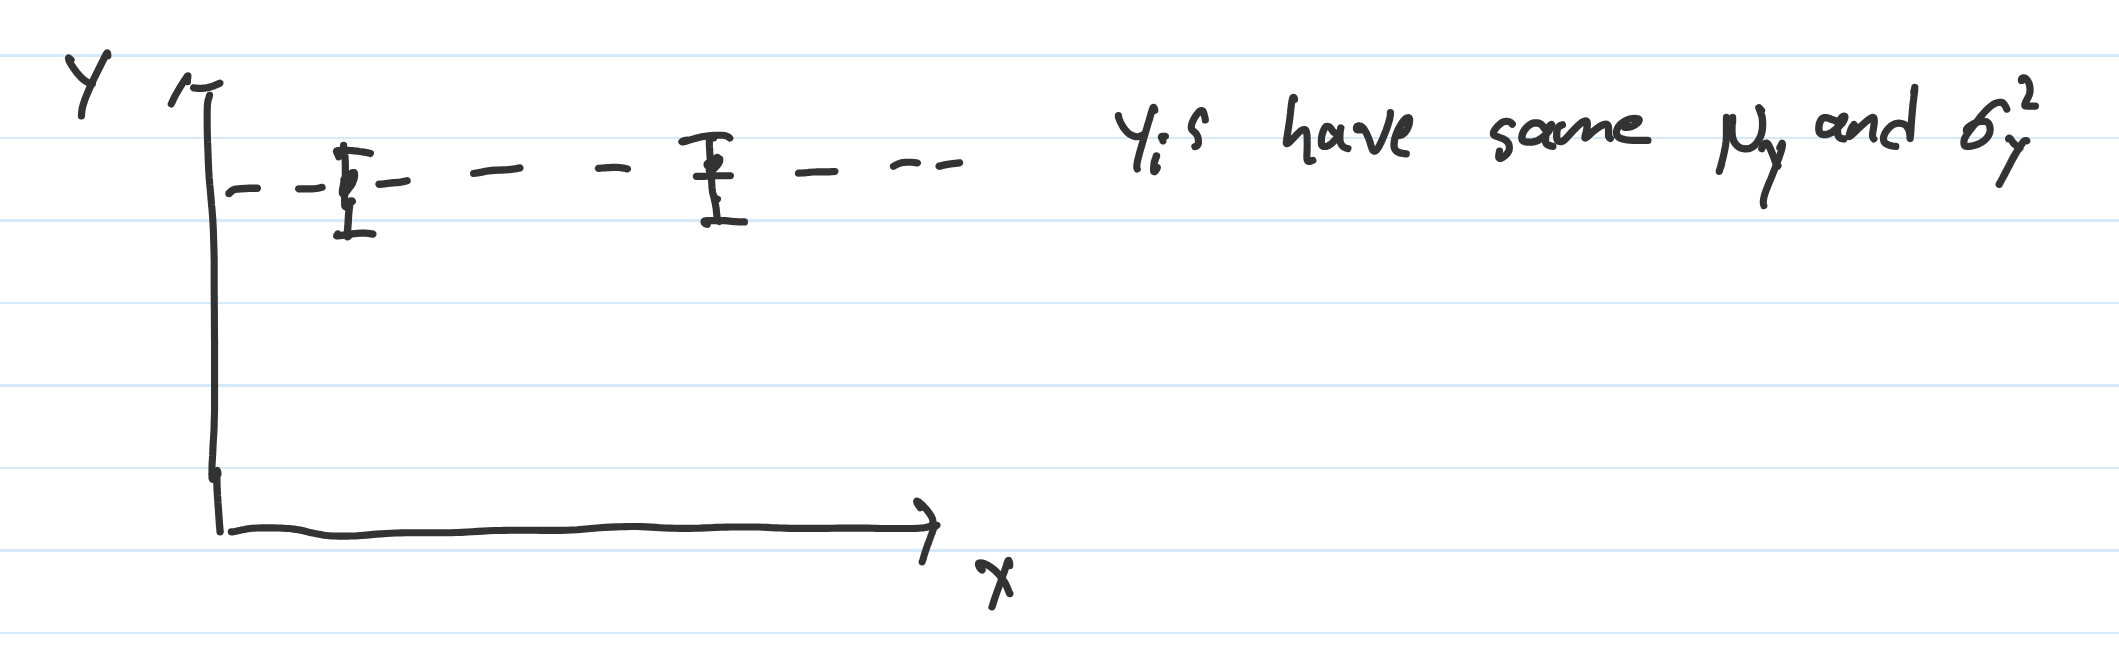
\includegraphics[width=0.8\linewidth]{Images/lec11-chisqu-example.png}

            $y_i$'s have some $N_y$ and $\sigma_y^2$.
\end{itemize}

\subsection{Two-Measurement Example and Correlated Variables}

\begin{itemize}
      \item Best estimator of the true $N$ is $\hat{y} = \frac{y_1 + y_2}{2}$.
            \[
                  \chi^2 = \left( \frac{y_1 - \hat{N}}{\sigma_y} \right)^2 +
                  \left( \frac{y_2 - \hat{N}}{\sigma_y} \right)^2
            \]
      \item Note:
            \[
                  y_1 - \hat{N} = \frac{1}{2} (y_1 - y_2)
            \]
            \[
                  y_2 - \hat{N} = \frac{1}{2} (y_2 - y_1)
            \]
      \item Where $z_1 = y_1 - y_2$, and $z_2 = y_2 - y_1$ such that $z_2 = -z_1$.
            \[
                  V(z_1, z_2) =
                  \begin{pmatrix}
                        1  & -1 \\
                        -1 & 1
                  \end{pmatrix}
            \]
      \item Determinant of $V$ is 0, so it is not invertible.
      \item Thus we effectively have only one independent variable.
\end{itemize}

\subsection{Residuals and Goodness of Fit}

\begin{itemize}
      \item Residual: $r_i = y_i - f_i(\vec{\theta})$.
      \item When talking about goodness of fit, people usually divide $\chi^2$ by the number of degrees of freedom (dof). If $\chi^2/\text{dof} \approx 1$, it is a good fit.
      \item What about residuals?

            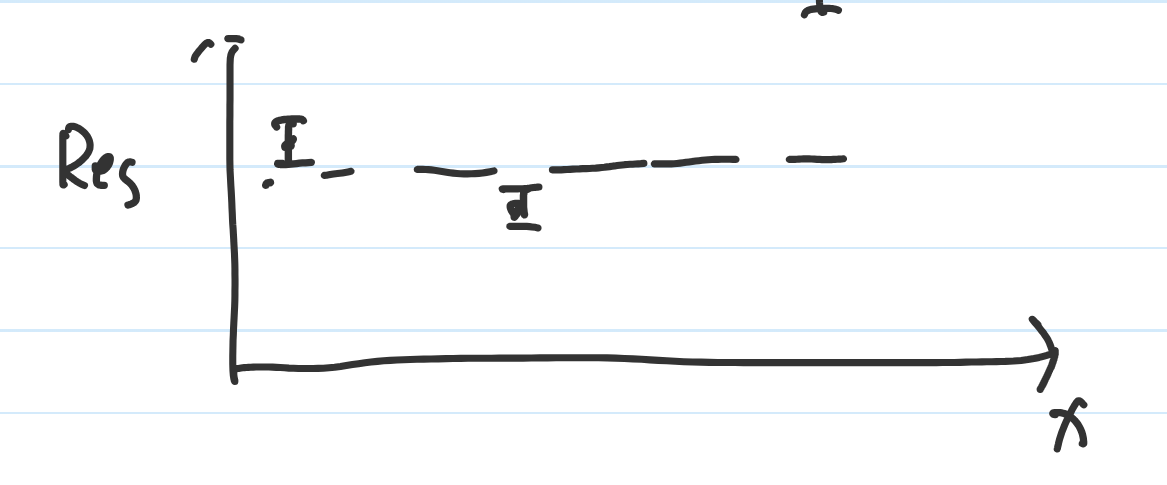
\includegraphics[width=0.5\linewidth]{Images/lec11-residual.png}

            Sometimes one weird data point can throw off the whole $\chi^2$ in unexpected ways, so it is important to check the residuals as well.
      \item If residuals are randomly scattered around 0, it indicates a good fit.
\end{itemize}

\subsection{Distribution of Estimators}

\begin{itemize}
      \item We have been talking about estimators, but we want values of the parameters.
      \item Suppose we perform a fit on a parameter with true value $a$.
      \item From fitting, we get different estimator values from different data sets.

            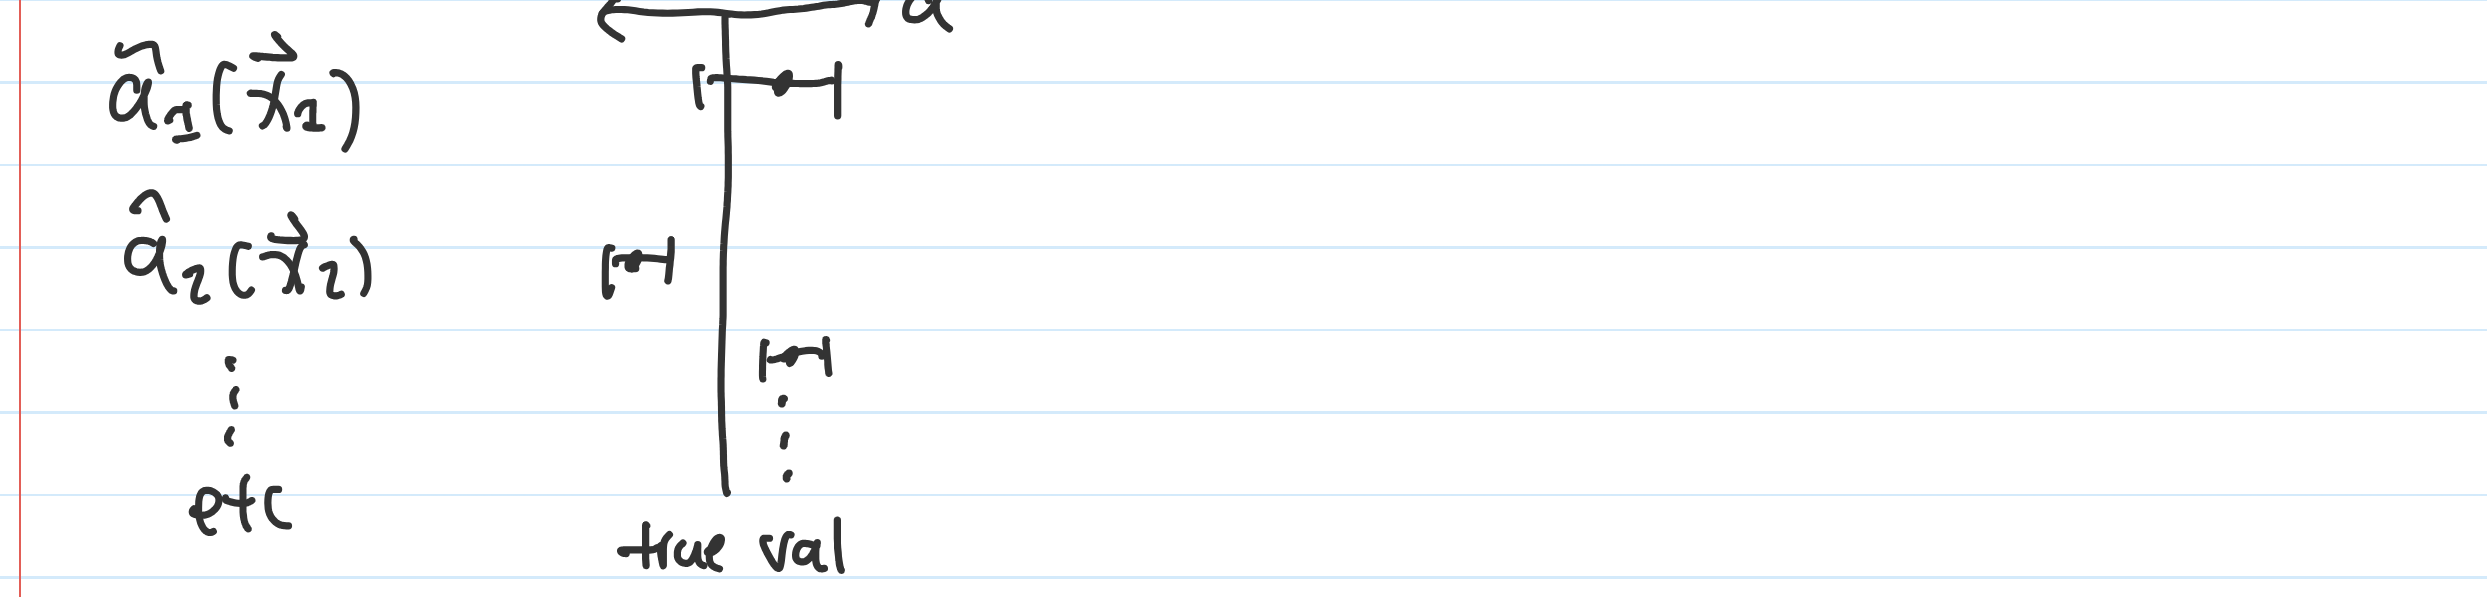
\includegraphics[width=0.5\linewidth]{Images/lec11-spread-est-vals.png}

      \item These estimates can be scattered over a range of values.
\end{itemize}

\subsection{Toy Monte Carlo Simulations for Estimator Distributions}

\begin{itemize}
      \item Toy Monte Carlo:

            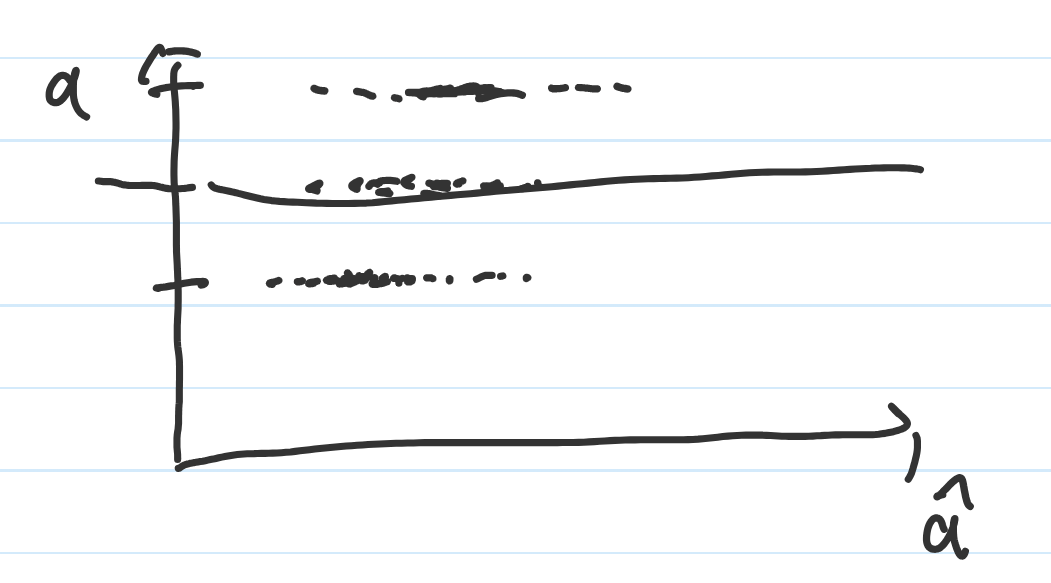
\includegraphics[width=0.6\linewidth]{Images/lec11-toy-monte-carlo.png}

      \item Often, the model is too complicated to get an analytic form of the estimator distribution.
            \begin{enumerate}
                  \item Pick a parameter $a$.
                  \item Generate many data sets according to the model with parameter $a$.
                  \item For each data set, compute the estimator $\hat{a}$.
                  \item Plot a histogram of $\hat{a}$.
                  \item Repeat steps 2–4 $n$ times.
                  \item Repeat step 1 $m$ times.
            \end{enumerate}
      \item For each $a$ value, we can determine e.g. 5\%, 90\%, and 5\% quantiles.

            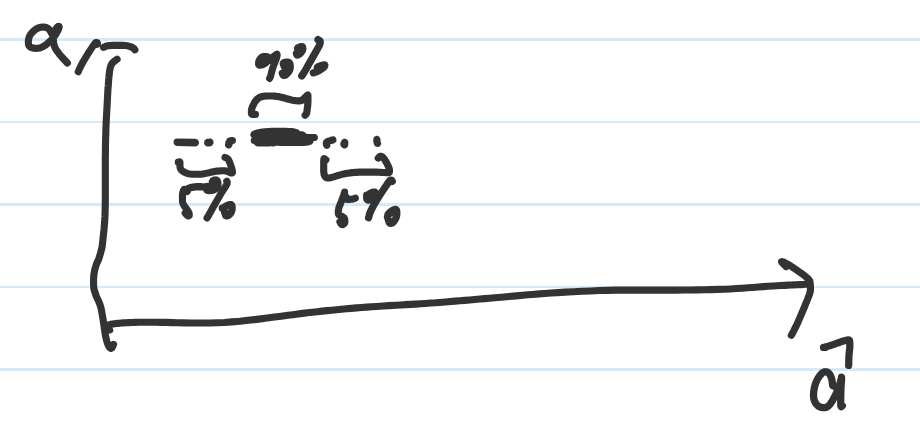
\includegraphics[width=0.6\linewidth]{Images/lec11-mc-intervals.png}

      \item We then connect these points.

            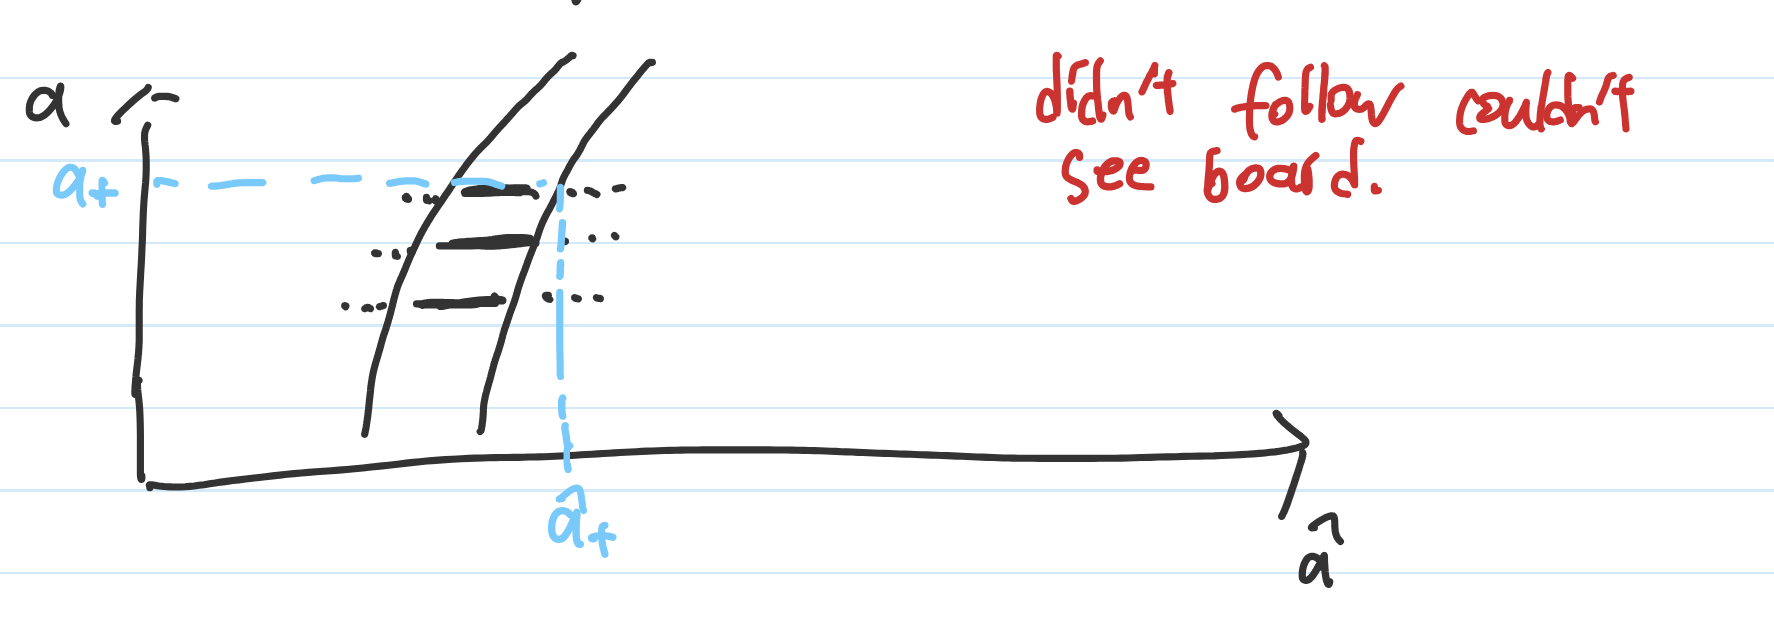
\includegraphics[width=0.6\linewidth]{Images/lec11-fit-connect.png}

      \item $P(a_{-} \leq a \leq a_{+}) = 0.90$.
            Coverage = fraction of time your prescription for the estimator interval contains the true value $a$.
      \item In other words, we find or choose $\hat{a}_{-}$ and $\hat{a}_{+}$ such that 90\% of the time, the true $a$ lies in our interval (corresponding to $a_{-}$ and $a_{+}$).
      \item The bias in all this is that we can really pick intervals however we want.

            
\includegraphics[width=0.6\linewidth]{Images/lec11-biased-intervals.png}
\end{itemize}

\subsection{Typical Applications of Least Squares Fitting}

\begin{itemize}
      \item Typical usage of Least Squares (LS):
            \begin{enumerate}
                  \item $x_i$, $y_i$, with known $\sigma_x$, and known $\sigma_y$ for $y_i$.

                        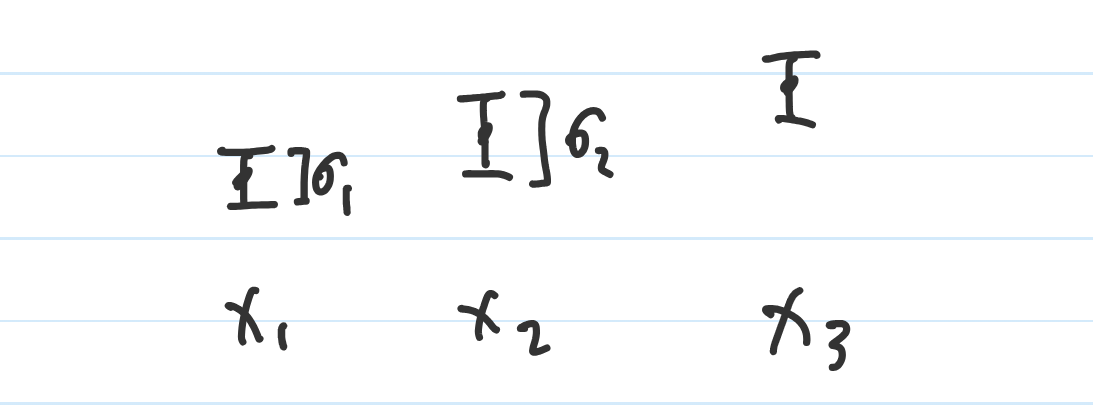
\includegraphics[width=0.4\linewidth]{Images/lec11-points.png}

                        If $y_i$'s are measured by a detector, we can determine $\sigma_i$ by analyzing the detector.
                  \item Histograms: i.e., measure $x$ on a coordinate, which can have resolution effects, etc., where $y =$ statistics of the number of events at the same $x$.

                        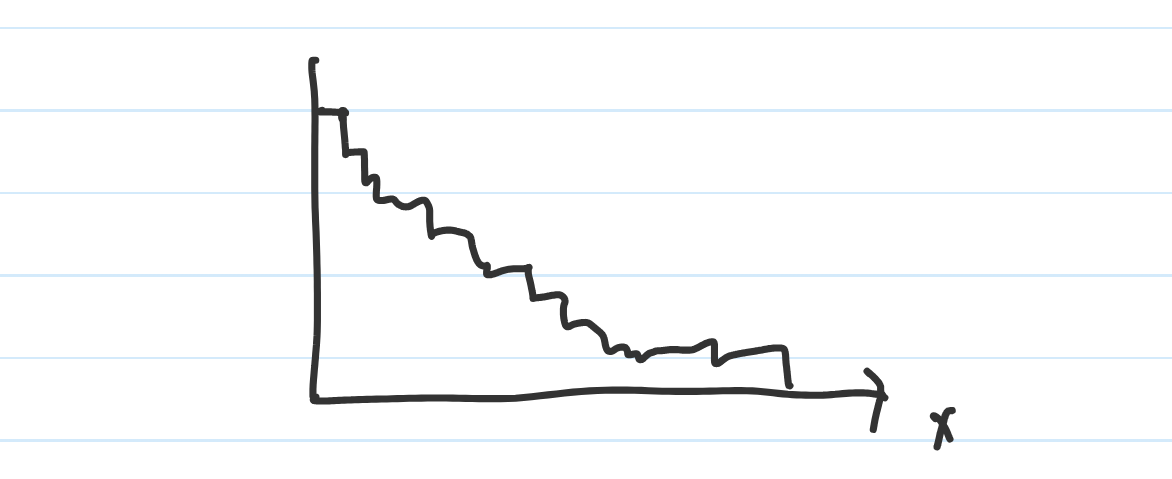
\includegraphics[width=0.4\linewidth]{Images/lec11-histogram.png}

                        Say the resolution has:

                        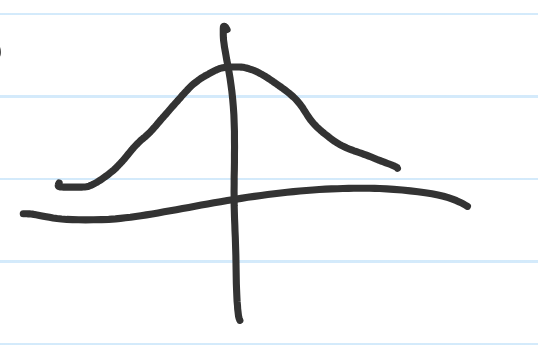
\includegraphics[width=0.4\linewidth]{Images/lec11-resolution.png}

                        so what you see is actually a convolution of the true distribution with the resolution function.

                        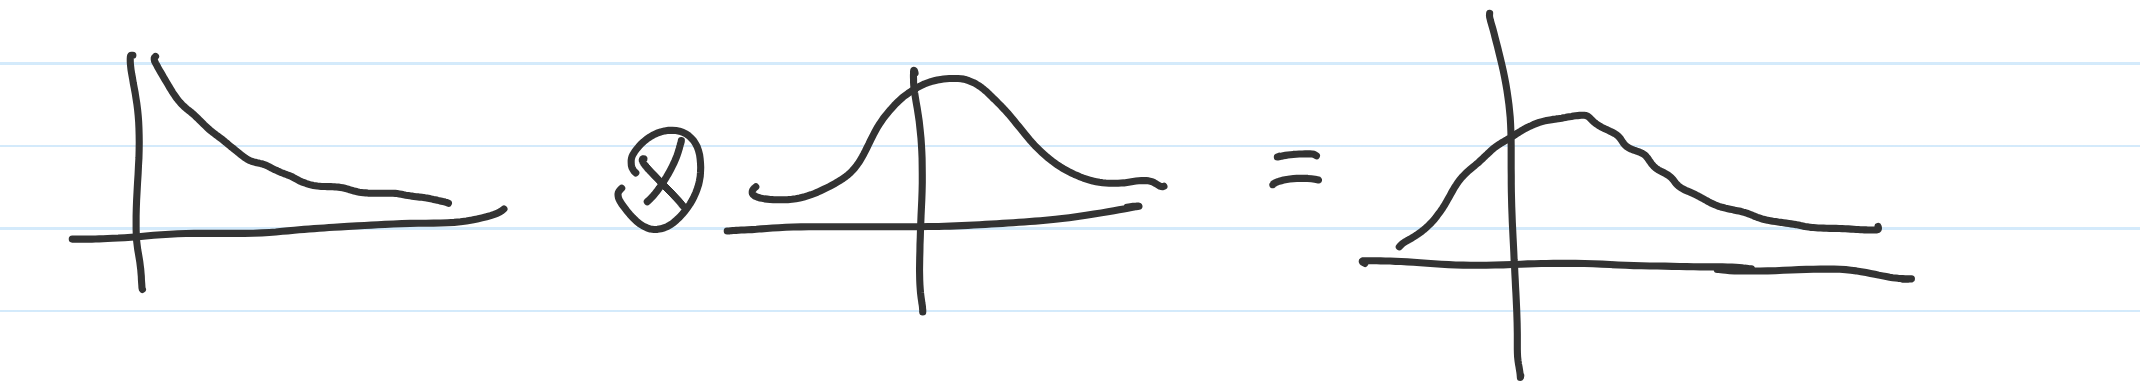
\includegraphics[width=0.4\linewidth]{Images/lec11-convolution.png}

                        So the fit should actually be an exponential $\circledast$ Gaussian in this case.

                        \[
                              \chi^2 = \sum_i \frac{(n_i - f_i(\theta))^2}{\sigma_i^2}
                        \]

                        Suppose we expect Poisson statistics:

                        \[
                              \sigma_i^2 = n_i
                        \]

                        Then the data are weighted by $n_i$:

                        \[
                              \text{Neyman } \chi^2 \equiv \sum_i \frac{(n_i - f_i(\theta))^2}{n_i}
                        \]

                        which is a modified least squares form.

                        Alternatively, it is sensible to say that the expected entries are given by our model:

                        \[
                              \Rightarrow \text{ use } f_i(\vec{\theta}) \text{ as the mean.}
                        \]

                        Therefore:

                        \[
                              \text{Pearson } \chi^2 \equiv \sum_i \frac{(n_i - f_i(\theta))^2}{f_i(\theta)}
                        \]

                        For Neyman $\chi^2$, if a bin is empty ($n_i = 0$) then it diverges.
                        Both Neyman and Pearson forms are biased in opposite ways.
                        One could use Neyman and Pearson together, but is it worth the effort?
            \end{enumerate}
\end{itemize}


\newpage
\section{Tuesday, October 21st 2025}

\subsection{Least-Squares Fits}

\begin{itemize}
      \item Usually we have data ($x_i, \, y_i \pm \sigma_i$). We want to fit a model $y = f(x; \, \theta)$ to the data.

            \[ \chi^2 = \sum_i \frac{(y_i - f(x_i; \, \theta))^2}{\sigma_i^2} \]

      \item Sometimes we are given $y = f(x)$ and sometimes we are given $x = g(y)$.

            \[ \chi^2 = \sum_i \frac{(x_i - g(y_i; \, \theta))^2}{\sigma_{x,i}^2} \]

            \[ \sigma_x = \left| \frac{dg}{dy} \right| \sigma_y \]

      \item Now that is the end of least-squared fits for a while.
\end{itemize}

\subsection{Unbinned Data and Likelihood Functions}

\begin{itemize}
      \item Now we move on to unbinned data.
      \item Idea is that you have some data drawn from some probability distribution $P(x;a)$
            \[ P(t) \sim \frac{1}{\tau} e^{-t/\tau} \]
      \item Data sample of size $n$: $\{x_1, \, x_2, \, \ldots, \, x_n\}$
      \item Form likelihood function:
            \[ \mathcal{L}(x_1, \, x_2, \, \ldots, \, x_n; \, a) = \prod_{i=1}^n P(x_i; \, a) \]
      \item This is equivalent to the probability of getting the data given the parameter $a$: $P(\vec{x} | a)$.
      \item Not a probability distribution in $a$! It is a function of $a$.
      \item Suppose we have an estimator $\hat{a}$ for $a$. Then the expectation value of the estimator is:
            \[ E[\hat{a}] = \int \hat{a}(\vec{x}) P(\vec{x}; \, a) d\vec{x} \]
      \item The maximum likelihood principle states that the best estimate for $a$ is the value $\hat{a}$ that maximizes $\mathcal{L}(\vec{x}; \, a)$:
            \[ \pdv{\mathcal{L}(\vec{x}; \, a)}{a} \Big|_{a = \hat{a}} = 0 \]
      \item Often easier to maximize $\ln \mathcal{L}$ since $\ln$ is monotonic:
            \[ \ln \mathcal{L}(\vec{x}; \, a) = \ln{ \prod_{i=1}^n P(x_i; \, a)} = \sum_{i=1}^n \ln P(x_i; \, a) \]
      \item Then we will find:
            \begin{enumerate}
                  \item max for $\ln \mathcal{L}(\vec{x}; \, a)$
                  \item min for $- \ln \mathcal{L}(\vec{x}; \, a)$
            \end{enumerate}
      \item ML estimators tend to be not unbiased, but consistent, often efficient.
            \[ \pdv{\ln \mathcal{L}(\vec{x}; \, a)}{a} \Big|_{a = \hat{a}} = 0 \]
\end{itemize}

\subsection{Example: Exponential Distribution}

\begin{itemize}
      \item Example: Exponential distribution
            \[ P(t; \, \tau) = \frac{1}{\tau} e^{-t/\tau} \]
            \[ \mathcal{L}(t_1, \, t_2, \, \ldots, \, t_n; \, \tau) = \prod_{i=1}^n \frac{1}{\tau} e^{-t_i/\tau} = \sum_{i=1}^n \ln\left( \frac{1}{\tau} e^{-t_i/\tau} \right) = - n \ln \tau - \frac{1}{\tau} \sum_{i=1}^n t_i \]
            \[ \pdv{\ln \mathcal{L}}{\tau} = 0 = - \frac{n}{\tau} + \frac{1}{\tau^2} \sum_{i=1}^n t_i \]
            \[ \hat{\tau} = \frac{1}{n} \sum_{i=1}^n t_i = \bar{t} \]
            This is unbiased.
      \item \[ E(\hat{\tau}) = \frac{1}{n} E(\sum_{i=1}^n t_i) = \frac{1}{n} \sum_{i=1}^n E(t_i) = \frac{1}{n} n \tau = \tau \]
\end{itemize}

\subsection{Example: Lifetime with Cutoff $T$}

\begin{itemize}
      \item (Not normalized $P$:)
            \[ P(t|\tau) = \begin{cases}
                        \frac{1}{\tau} e^{-t/\tau} / e^{-T/\tau} & 0 \geq t \geq T  \\
                        0                                        & \text{otherwise}
                  \end{cases} \]
      \item Now must normalize! $\sum_{t=T}^{\infty} P(t|\tau) = 1$
            \[ P(t|\tau) = \frac{1}{(1-e^{-T/\tau}) \tau} e^{-t/\tau} \]
      \item Log-likelihood:
            \[ \ln \mathcal{L} = \sum_{i=1}^n \left[ \ln\left( (1-e^{-T/\tau}) \tau \right) \right] - \frac{1}{\tau} \sum_{i=1}^n t_i \]
            \[ = -n \ln (1-e^{-T/\tau}) - n \ln \tau - \frac{1}{\tau} \sum_{i=1}^n t_i \]
      \item Set derivative to zero:
            \[ \pdv{\ln \mathcal{L}}{\tau} = 0 \]
            \[ \pdv{\ln \mathcal{L}}{\tau} = \frac{-n (-e^{-T/\tau}) (\frac{T}{\tau^2})}{(1-e^{-T/\tau})} - \frac{n}{\tau} + \frac{1}{\tau^2} \sum_{i=1}^n t_i = 0 \]
\end{itemize}

\subsection{Example: Multiple Gaussian Measurements}

\begin{itemize}
      \item Multiple measurements of some quantity:
            \[ P(x | \mu, \sigma) = \frac{1}{\sqrt{2 \pi} \sigma} e^{-(x - \mu)^2 / 2 \sigma^2} \]
            \[ \ln \mathcal{L} = - \sum_i \ln (\sqrt{2 \pi}) - \sum_i \ln \sigma - \frac{1}{2} \sum_i \frac{(x_i - \mu)^2}{\sigma^2} \]
            \[ \pdv{\ln \mathcal{L}}{\mu} = 0 = \frac{-1}{2} (-2) \sum_i \frac{(x_i - \mu)}{\sigma^2} \]
            \[ = \frac{1}{\sigma^2}  \sum_i (x_i - \hat{\mu}) = 0 \]
            \[ \sum_i x_i = n \hat{\mu} \Rightarrow \hat{\mu} = \frac{1}{n} \sum_i x_i = \bar{x} \]
      \item Now for $\sigma$:
            \[ \pdv{\ln \mathcal{L}}{\sigma}\Big|_{\hat{\sigma}, \hat{\mu}} = 0 = -\frac{n}{\sigma}- \frac{1}{2} \left(\frac{-2}{\sigma^3} \right) \sum_i (x_i - \mu)^2 \]
            \[ -n \hat{\sigma^2} + \sum_i (x_i - \hat{\mu})^2 = 0 \]
            \[ \hat{\sigma^2} = \frac{1}{n} \sum_i (x_i - \hat{\mu})^2  = \frac{1}{n} \sum_i (x_i - \bar{x})^2 \]
      \item This is a biased estimator for $\sigma^2$. Unbiased is with $1/(n-1)$.
\end{itemize}

\subsection{Properties of the Maximum-Likelihood Estimator}

\begin{itemize}
      \item This next stuff is not really testable but can be interesting to see where it comes from.
      \item To avoid confusion call $a_0$ the true value of $a$.
      \item We have $\mathcal{L}(\vec{x}; \, a)$ and we want to know how well $\hat{a}$ estimates $a_0$.
            \[ \pdv{\ln \mathcal{L}(\vec{x}; \, a)}{a} \Big|_{a = \hat{a}} = 0 \]
      \item Taylor expand around $a_0$:
            \[ f(\hat{a}) = f(a_0) + f'(a_0) (\hat{a} - a_0) + \frac{1}{2} f''(a_0) (\hat{a} - a_0)^2 + \ldots \]
      \item So we have:
            \[ \pdv{\ln \mathcal{L}(\vec{x}; \, a)}{a} \Big|_{a = \hat{a}} = \pdv{\ln \mathcal{L}(\vec{x}; \, a)}{a} \Big|_{a = a_0} + (\hat{a} - a_0) \pdv[2]{\ln \mathcal{L}(\vec{x}; \, a)}{a} \Big|_{a = a_0} + \ldots = 0 \]
      \item For $n\rightarrow \infty$, $\hat{a} \rightarrow a_0$ (consistent estimator), so we can neglect higher order terms.
            \[ \pdv{\ln \mathcal{L}(\vec{x}; \, a)}{a} \Big|_{a = a_0} \rightarrow \pdv{\ln \mathcal{L}(\vec{x}; \, a)}{a} \Big|_{a = \hat{a}} = 0 \]
\end{itemize}

\newpage
\section{Lecture 13}

Thursday, October 23rd 2025

\subsection{Definition of the Likelihood Function}

\begin{itemize}
    \item Likelihood
          \[ \mathcal{L}(\vec{x}|\theta) = \text{probability of x and not theta} \]
    \item Model $\vec{\theta}$ with $p(\vec{x}|\vec{\theta})$
          \[ \mathcal{L} = \prod_{i=1}^{N} p(x_i|\vec{\theta}) \]
          \[ \ln \mathcal{L} = \sum_{i=1}^{N} \ln p(x_i|\vec{\theta}) \]
\end{itemize}

\subsection{Maximum Likelihood Estimation (MLE)}

\begin{itemize}
    \item Maximize likelihood to get best estimate of $\vec{\theta}$. Choose $\hat{\theta}$ such that:
          \[ \hat{\theta} = \text{argmax}_{\vec{\theta}} \mathcal{L}(\vec{x}|\vec{\theta}) \]
          \[ \pdv{\ln \mathcal{L(\vec{\theta})}}{\theta} \Big|_{\hat{\theta}} = 0 \]
\end{itemize}

\subsection{Quadratic Approximation of the Log-Likelihood}

\begin{itemize}
    \item Shape of $\vec{a}$ distribution: $\ln \mathcal{L}(a)$ around $\hat{a}$ is approximately quadratic.
    \item True $a = \hat{a}$; expand about $a_0$:
    \item Taylor expansion:
          \[ f(a) = f(a_0) + (\hat{a} - a_0) f'(a_\star) \qquad \text{where } a_{\star} \text{ is between } \hat{a} \text{ and } a_0 \]
    \item So, for $f = \pdv{\ln \mathcal{L}(a)}{a}$:
          \[ 0 = \pdv{\ln \mathcal{L}(a)}{a} \Big|_{a_0} + (\hat{a} - a_0) \pdv[2]{\ln \mathcal{L}(a)}{a} \Big|_{a_{\star}} \]
\end{itemize}

\subsection{Asymptotic Limit and Expectation Relation}

\begin{itemize}
    \item Large $n$ for consistent $\hat{a} \to a_0$:
          \[ \lim_{n \to \infty} \pdv[2]{\ln \mathcal{L}(a)}{a} \Big|_{a_{\star}} = \lim_{n \to \infty} \sum_i \pdv[2]{\ln p(x_i|a)}{a} \Big|_{a_{\star}} \approx \lim_{n} n \int p(x|a) \pdv[2]{\ln p(x|a)}{a} \Big|_{a_{\star}} dx \]
    \item Sum over samples $x_i$ drawn from $p(x|a)$:
          \[ = \lim_{n \to \infty} n E\left( \pdv[2]{\ln p(x|a)}{a} \Big|_{a_{\star}} \right) \]
          \[ = E \left( \pdv[2]{\ln \mathcal{L}}{a} \Big|_{a_{\star}} \right) \]
          \[ \hat{a} - a_0 = - \frac{\pdv{\ln \mathcal{L}(a)}{a} \Big|_{a_0}}{E\left( \pdv[2]{\ln \mathcal{L}}{a} \Big|_{a_{\star}} \right)} \]
          \[ 0 = \pdv{\ln \mathcal{L}(a)}{a} \Big|_{a_0} + (\hat{a} - a_0) \pdv[2]{\ln \mathcal{L}(a)}{a} \Big|_{a_{\star}} \]
\end{itemize}

\subsection{Normalization of the Likelihood Function}

\begin{itemize}
    \item The likelihood is normalized:
          \[ \int \mathcal{L}(\vec{x}|a) d\vec{x} = 1 \]
          \[ \Rightarrow \int \pdv{\mathcal{L}(\vec{x}|a)}{a} d\vec{x} = 0 \]
    \item Relation between $\mathcal{L}$ and $\ln \mathcal{L}$:
          \[ \pdv{\mathcal{L}}{a} = \pdv{\ln \mathcal{L}}{a} \mathcal{L} \]
          \[ \pdv{\ln \mathcal{L}}{a} = \sum_{i=1}^{n} \pdv{\ln p(x|a)}{a} \]
\end{itemize}

\subsection{Gaussian Approximation via the Central Limit Theorem}

\begin{itemize}
    \item The sum of $n$ variables with zero mean:
    \item By the Central Limit Theorem, for large $n$, $\pdv{\ln \mathcal{L}}{a}$ is Gaussian with mean 0.
          \[ \boxed{E\left(\pdv[2]{\ln \mathcal{L}}{a} \right) = - E \left( \left( \pdv{\ln \mathcal{L}}{a} \right)^2 \right) } \]
\end{itemize}

\subsection{Variance of the Estimator and the Fisher Information}

\begin{itemize}
    \item Variance of $\hat{a} - a_0$:
          \[ \text{Var}(\hat{a} - a_0) = \frac{\text{Var}\left( \pdv{\ln \mathcal{L}(a)}{a} \Big|_{a_0} \right)}{\left( E\left( \pdv[2]{\ln \mathcal{L}}{a} \Big|_{a_{\star}} \right) \right)^2} \]
          \[ = \frac{E\left( \left( \pdv{\ln \mathcal{L}(a)}{a} \Big|_{a_0} \right)^2 \right)}{\left( E\left( \pdv[2]{\ln \mathcal{L}}{a} \Big|_{a_{\star}} \right) \right)^2} \]
          \[ = -\frac{E\left( \pdv[2]{\ln \mathcal{L}}{a} \Big|_{a_0} \right)}{\left( E\left( \pdv[2]{\ln \mathcal{L}}{a} \Big|_{a_{\star}} \right) \right)^2} \]
    \item When $n \to \infty$, $a_{\star} \to a_0$ and $\hat{a} \to a_0$:
          \[ \boxed{\text{Var}(\hat{a}) = -\frac{1}{E\left( \pdv[2]{\ln \mathcal{L}}{a} \Big|_{a_0} \right)} } \]
    \item Fisher Information matrix:
          \[ E\left( \pdv[2]{\ln \mathcal{L}}{a} \right) \]
    \item For large $n$, $\hat{a} \to a_0$. Estimate $E(\cdot)$ by the observed value:
          \[ \pdv[2]{\ln \mathcal{L}}{a} \Big|_{\hat{a}} \]
    \item So the estimate of variance of $\hat{a} - a_0$ is:
          \[ \boxed{\text{Var}(\hat{a}-a_0) = -\frac{1}{\pdv[2]{\ln \mathcal{L}}{a} \Big|_{\hat{a}}} } \]
\end{itemize}

\subsection{Taylor Expansion Near the Maximum Likelihood Estimate}

\begin{itemize}
    \item Taylor expansion again:
          \[ \pdv{\ln \mathcal{L}(a)}{a} = \cancelto{0}{\pdv{\ln \mathcal{L}(a)}{a} \Big|_{\hat{a}}} + (a - \hat{a}) \pdv[2]{\ln \mathcal{L}(a)}{a} \Big|_{\hat{a}} + \ldots \]
          where $\pdv[2]{\ln \mathcal{L}(a)}{a} \Big|_{\hat{a}} = -\frac{1}{V(\hat{a})}$
          \[ \frac{-(a-\hat{a})}{V(\hat{a})} + \ldots \]
    \item Note that $V(\hat{a} - a_0) = V(\hat{a})$ because $a_0$ is constant and does not change the variance (it just shifts the distribution).
    \item So,
          \[ \ln \mathcal{L}(a) = \ldots \text{ missed this part} \]
\end{itemize}

\subsection{Goodness of Fit and the Kolmogorov–Smirnov Test}

\begin{itemize}
    \item Note that the value you get from the maximum likelihood does not give information on how good the fit is—it is just relative to other values of the parameters.
    \item Kolmogorov–Smirnov test for goodness of fit (KS):
          \begin{enumerate}
              \item Order data points $\{t_i\}$ such that $t_0 \leq t_1 \leq t_2 \leq \ldots \leq t_N$
              \item Form an accumulator $F$ (same model CDF $C$).
          \end{enumerate}
    \item Metric:
          \[ \text{max}|F(t_i) - C(t_i)| \]
\end{itemize}

\end{document}